\documentclass{article}
%\documentclass[draft]{article}
\usepackage{graphicx}
%\usepackage[draft]{graphicx}
\graphicspath{{figs}{notebooks}{.}}
\usepackage{hyperref}
\usepackage{amsmath}
\usepackage{amsfonts}
\usepackage{amssymb}
\usepackage[margin=1in]{geometry}
\usepackage{comment}
\usepackage{color}
%\usepackage[%
%filename ,%
%content={no image available}
%]{draftfigure}

\title{Denoising in Microscopy Imaging}

\author{Vicente González-Ruiz and José Jesús Fernández Rodríguez}

\begin{document}
\maketitle

\begin{abstract}
%{{{

  Microscopy of biological specimens is used in biotechnology to
  visualize small specimens (including their internal structures) that
  cannot be seen with the naked eye. For this, some kind of
  interaction between the specimens and a source of energy must exist
  (the specimen must be irradiated). In light miscroscopy (optical
  micoscopes), the sample is irradiated with visible light or a
  laser. In electron microscopy we use beans of electrons that can
  pass through the sample (TEM (Transmission Electron Microscopy)) or
  bounce on the sample (SEM (Scanning Electron Microscopy)). X-rays
  and ions can be also used (the smaller the wavelength of the bean,
  the higher the resolution). Unfortunately, the radiation also
  degrades the samples, specially in the case of biological
  specimens. To minimize this degradation, the radiation doses are
  minimized, generating low signal-to-noise ratio images. In this
  report, we describe, evaluate, and compare several image denoising
  algorithms commonly used in microscopy.

%}}}
\end{abstract}

\tableofcontents

\section*{Definitions and notation}
%{{{

\begin{tabular}{ll}
  $x$ & A scalar value (e.g., a value of a pixel of a grayscale image) \\
  $s(t)$ & A (continuous) signal as a function of time \\
  $s[n]$ & A discrete signal (only) defined at instants of time $tn, n\in\mathcal{Z}, t>0$ \\
  $\mathbf{s}$ & A digital (discrete and finite) signal (e.g., an image) \\
  $\mathbf{s}_{i}$ & The $i$-th element of $\mathbf{s}=\{\mathbf{s}_{i}\}_{i=0}^{N-1}=\{\mathbf{s}_{i}\}$ \\
  %$A[b]$ & The $b$-th element of the sampled version of $A(b)$ \\
  $\{i\}$ & The set $i$ \\
  $\mathbf{s}_{\{i\}}$ & The elements of $\mathbf{s}$ with indices $\{i\}$ \\
  $\mathbf{s}_{\href{https://numpy.org/doc/stable/user/basics.indexing.html#slicing-and-striding}{y,:}}$ & The $y$-th row of the 2D signal (image) $\mathbf{s}$ \\
  $\mathbf{s}_{:,x}$ & The $x$-th column of the image $\mathbf{s}$ \\
  $\mathbf{s}_{y,x}$ & The pixel $(y,x)$ of the image $\mathbf{s}$ \\
  %$\mathbf{x}^{(i)}$ & The $i$-th real-noisy instance of the signal $\mathbf{x}$ \\
  $\mathbf{s}^{()}$ & A instance of $\mathbf{s}$, possibly noisy \\
  $\mathbf{s}^{(i)}$ & The $i$-th instance of the signal $\mathbf{s}$ \\
  $\tilde{\mathbf{s}}^{(I)}$ & Approximation to $\mathbf{s}$ using $I$ instances \\ 
  $\overline{\mathbf{s}}$ & A mean of the samples of $\mathbf{s}$ \\ 
  $\href{https://docs.python.org/3/library/functions.html#len}{\text{len}}(\mathbf{s})$ & $=\mathbf{s}.\href{https://numpy.org/doc/stable/reference/generated/numpy.ndarray.size.html}{\mathsf{size}}$ Number of elements in $\mathbf{s}$ \\
  $\href{https://numpy.org/doc/stable/reference/generated/numpy.shape.html}{\text{shape}}(\mathbf{s})$ & ($=\mathbf{s}.{\mathsf{shape}}$) Shape of $\mathbf{s}$ \\
  $\text{rank}(\mathbf{s})$ & ($=\mathbf{s}.\mathsf{rank}=\text{len}(\mathbf{s}.\mathsf{shape})$) Dimensionality of $\mathbf{s}$ \\
  $\mathsf{\href{https://docs.python.org/3/library/functions.html\#func-range}{range}}(s)$ & $=\{0, 1, \cdots, s-1\}$ \\
  $\mathsf{\href{https://numpy.org/doc/stable/reference/generated/numpy.zeros_like.html}{zeros\_like}}(\mathbf{s})$ & $=\{0\}_{i=0}^{\mathbf{s}.\mathsf{size}-1}$ \\
  % $|\mathbf{X}_i|$ & The absolute value of $\mathbf{X}_i$ \\
  $\alpha\mathbf{s}$ & $=\{\alpha\mathbf{s}_i\}$ (scalar multiplication) \\
  $\mathbf{x}+\mathbf{y}$ & $=\{\mathbf{x}_i + \mathbf{y}_i\}$ (Hadamard addition) \\ 
  $\mathbf{x}\mathbf{y}$ & $=\{\mathbf{x}_i\mathbf{y}_i\}$ (Hadamard product) \\ 
  $\mathcal{N}$ & The normal distribution \\ 
  $\mathcal{P}$ & The Poisson distribution \\
  $\mathbf{s}\sim\mathcal{N}$ & The elements of $\mathbf{s}$ follows a normal distribution \\
  $\mathbf{s}_{\mathcal{N}}$ & The same as $\mathbf{s}\sim\mathcal{N}$ \\
  $\Pr(\mathbf{x}=a)$ & Probability that a $\mathbf{s}_i$ takes the value $a$ \\
  $\Pr(\mathbf{x}=a, \mathbf{y}=b)$ & $\Pr(\mathbf{x}=a)$ and $\Pr(\mathbf{y}=b)$ (joint probability)  \\
  $\mathrm{Su}(\mathbf{s})$ & $=\{x\in\mathbb{R}|\Pr(\mathbf{s}=x)>0\}$ (support of $\mathbf{s}$)\\
  $\Pr(A|B)$ & Conditional probability of $A$ given $B$ \\
  $\mathbb{E}(\mathbf{s})$ & Expectation of $\mathbf{s}$ \\
  $||\mathbf{s}||_2$ & $L_2$ norm of $\mathbf{s}$ \\
  $f_s$ & Sampling frequency \\
  $\mathcal{F}$ & The (forward) Fourier transform ($\mathcal{F}(\mathbf{s})=\mathbf{S}$) \\
  $\mathcal{F}^{-1}$ & The inverse Fourier transform ($\mathcal{F}^{-1}(\mathbf{S})=\mathbf{s}$) \\
  $\cdot^*$ & the complex conjugate of $\cdot$ \\
  $\mathbf{x}*\mathbf{y}$ & $=\mathcal{F}^{-1}(\mathcal{F}(\mathbf{x})\mathcal{F}(\mathbf{y}))=\mathcal{F}^{-1}(\mathbf{X}\mathbf{Y})$ (convolution) \\
  $A(b)$ & $A$ depends on (parameter) $b$ \\
  $A.b$ & The $b$ component of the data structure $A$ \\
  $(A)b$ & First $A$, then $b$ 
\end{tabular}

%}}}

\section{Imaging techniques}
%{{{

The most common imaging techiniques used in microscopy are:

\begin{enumerate}
\item \textbf{Light microscopy (LM)}: Uses visible light and optical
  lenses to magnify specimens. \textbf{Fluorescence microscopy} and
  \textbf{confocal microscopy} are subtypes of LM where the specimens emit
  light after have being excited by a source of light. Typical
  resolution: 200 nm.
\item \textbf {Electron microscopy (EM)}: Uses electron beams instead
  of light for imaging, allowing much higher resolution (down to
  sub-nanometer scale). Two main techniques exist:
  \textbf{Transmission electron microscopy (TEM)} where the electrons
  pass through thin specimens, providing internal structural details,
  and \textbf{scanning electron microscopy (SEM)}, where the electrons
  bounce off the surface, showing the 3D surface morphology.
\item \textbf{Atomic force microscopy (AFM)}: A form of scanning probe
  microscopy that maps the surface of a specimen with a nano-scale
  mechanical probe.
\end{enumerate}

%}}}

\section{Signals and random variables}
Mathematically, we can model signals as random variables. A random
variable is a mathematical formalization of a quantity or object which
depends on random events. When more than one value (a vector) is
generated in one of these envents, we can establish a similar
connection between multicomponent signals and random vectors. Random
variables (and therefore monocomponent signals) will be denoted with
bold-faced symbols, such as $\mathbf{x}$. Random vectors
(multicomponent signals) will be denoted as
$\overrightarrow{\mathbf{x}}$.

Statistically, random variables can be described throught the mean and
the variance and the corresponding distribution. Random vectors
require a mean for each component, a covariance matrix, and a
multivariate distribution.

\section{Common sources of noise}
%{{{

There are three main sources of noise, in microscopy imaging: (1)
\emph{dark noise} which corresponds to the electronic noise generated
by the thermal agitation of electrons, (2) \emph{photon noise} (or
shot noise) that is generated by the fluctuations in the number of
photons sensed at a given signal exposure level, and (3) the
\emph{readout noise}, generated by the non-perfectness of the output
electronic amplifiers used in the process of converting photon or
electron accumulations into voltages. Therefore, the level of noise
depends on the exposure time and experimental conditions affecting the
sensors such as temperature, among other capturing parameters. Dark
and photon noises are modeled as a Poisson distribution
$\mathcal{P}(\lambda)$, where $\lambda$ represents the average dark
flux. Readout noise is modeled as zero-mean additive white Gaussian
noise \cite{meiniel2018denoising,zhou2020wirtinger}.

\begin{comment}
\subsection{Quantization noise}
%{{{

All digital capturing devices generate quantization noise which is
usually modeled as additive zero-mean uniform noise
(${\mathbf N}\sim{\mathcal U}(c)$). The PDF (Probability Density
Function) is defined by
\begin{equation}
  f(x; c) = \Pr({\mathbf N}^{(i)}_j{=}x) \triangleq \begin{cases}
    \frac{1}{2c} & \text{for } -c \le x \le c, \\[8pt]
    0 & \text{for } x < c \ \text{ or } \ x > -c,
  \end{cases}
\end{equation}
$x$ and $f$ continuous, where $\Pr(\cdot)$ represents the
probability of $\cdot$, and $c$ controls the amplitude of the
noise. Notice that in this case, $\overline{\mathbf{N}}^{(i)}=0$ and
therefore, $\overline{\mathbf N}={\mathbf 0}$ (see
Eq.~\ref{eq:noise_expectation_2}). 

%}}}
\end{comment}

\subsection{Zero-mean Additive White Gaussian (ZAWG) noise}
%{{{

A noisy signal $\hat{\mathbf s}$ corrupted by \href{https://en.wikipedia.org/wiki/Gaussian_noise}{Zero-mean Additive White Gaussian (ZAWG) noise} can be modeled as
\begin{equation}
  \hat{\mathbf s} = {\mathbf s} + {\mathbf n}_{{\mathcal N}(\sigma)},
  \label{eq:AWG_noise_model}  
\end{equation}
where $\mathbf{s}$ is the \emph{clean} signal (without noise, ground
truth usually unknown),
and ${\mathbf n}$ is a tensor of random samples,
where, for the ZAWG noise case,
${\mathbf n}\sim{\mathcal N}(\mu=0,\sigma)$, with PDF (probability density
function)
\begin{equation}
  \Pr({\mathbf n}{=}x) = \frac 1 {\sigma\sqrt{2\pi}} e^{-\frac{x^2}{2\sigma^2} }.
\end{equation}
In theory, $x\in\mathbb{R}$ can be continuous, although in our
context, $x$ is a signal sample and therefore, discrete,
$\mu\in\mathbb{R}$ is the mean, and $\sigma\in\mathbb{R}$ represents
the standard deviation of the noise. Notice that this is a
signal-independent model because nothing can said about ${\mathbf n}$
known $\hat{\mathbf s}$, except that
\begin{equation}
  \Pr(\mathbf{n}{=}n|\hat{\mathbf{s}}) = \Pr(\mathbf{n}{=}n).
\end{equation}

By definition, the spectrum of AWG noise is flat. Therefore, the
performance of a pure low-pass filter denoiser will depend on the
shape of the spectrum of $\mathbf{s}$.

%}}}

\subsection{Poisson noise}
%{{{

Poisson noise
\href{https://en.wikipedia.org/wiki/Poisson_distribution}{is defined}
to have a PMD (Probability Mass Distribution)\footnote{Also called
  discrete PDF.}
\begin{equation}
  \Pr({\mathbf n}{=}k) = \frac{\mathbf{\lambda}^ke^{-\mathbf{\lambda}}}{k!},
  \label{eq:PN}
\end{equation}
which describes the probability of $k\in\mathbb{n}$ events ocurring
within an observed interval (of time, for example), when, on average
(arithmetic mean) we have ${\mathbf \lambda}\in\mathbb{R}$ events in
such interval. Using
\href{https://numpy.org/doc/stable/reference/random/generated/numpy.random.poisson.html#numpy-random-poisson}{\texttt{numpy.random.poisson}},
which inputs $\mathbf{s}$, we can generate Poisson noise with
\begin{equation}
  \hat{\mathbf{s}} = \frac{\mathbf{n}(\mathbf{s})}{\gamma},~\mathbf{n}\sim\mathcal{P}(\lambda=\gamma\mathbf{s}),
\end{equation}
where $\gamma$ controls the standard deviation (the higher $\gamma$,
the smaller the deviation from the $\mathbf{s}$ values). As can be
seen, this is a signal-dependent model because the brighter parts of
$\hat{\mathbf s}$ will have a higher mean and variance\footnote{The
  mean and variance of a Poisson law are both equal to $\lambda$.},
and therefore a higher noise level \cite{meiniel2018denoising}.

%}}}

\subsection{Mixed Poisson-Gaussian (MPG) noise}
%{{{

A more realistic noise model in microscopy consists in a combination
of both Poisson and ZAWG noise, which is commonly called mixed
Poisson-Gaussian noise \cite{meiniel2018denoising}. In this
case, we have that
\begin{equation}
  \Pr({\mathbf n}{=}k) = \frac{e^{-\lambda}}{\sqrt{2\pi}\sigma}\sum_{p=0}^{\infty}\frac{\lambda^p}{p!} e^{-\frac{\gamma p - k}{2\sigma^2}},
  \label{eq:PN}
\end{equation}
and that
\begin{equation}
  \hat{\mathbf s} = (1-\alpha)(\mathbf{s} + {\mathbf s}_{\mathcal{N}(\sigma)}) + \alpha{\mathbf n}_{\mathcal{P}(\lambda=\gamma\mathbf{s})}/\gamma,
  \label{eq:MPG_noise_model} 
\end{equation}
where $\alpha\in[0,~1]$ controls the ratio of both types of
noise. Therefore, for $\alpha > 0$,\footnote{If $\sigma=0$ and
  $\alpha=0$, both types of noise vanish and
  $\hat{\mathbf{s}}=\mathbf{s}$.} the noise is signal-dependent and
it's spectrum resembles the spectrum of $\mathbf{x}$. By default, in
our experiments, $\alpha=0.5$.

%}}}

% A. Foi, M. Trimeche, V. Katkovnik, and K. Egiazarian.
% Practical Poissonian-Gaussian noise modeling and fitting for
% single-image raw-data. IEEE Transactions on Image Pro-
% cessing, 17(10):1737–1754, 2008.

%\subsection{Noise estimation}
%{{{

% Makitalo and A. Foi. Optimal inversion of the generalized
% Anscombe transformation for Poisson-Gaussian noise. IEEE
% Transactions on Image Processing, 22(1):91–103, 2013.
% https://link.springer.com/chapter/10.1007/978-3-030-87231-1_33

% A. Foi, M. Trimeche, V. Katkovnik, and K. Egiazarian.
% Practical Poissonian-Gaussian noise modeling and fitting for
% single-image raw-data. IEEE Transactions on Image Pro-
% cessing, 17(10):1737–1754, 2008.

%}}}

%\subsection{Anscombe transform and gneralized Anscombe transformation (GAT)}
%{{{

% Using a nonlinear variance-stabilizing transformation (VST) to convert the
% Poisson-Gaussian denoising problem into a Gaussian noise
% removal problem. The VST is able to remove the signal-dependency of
% the Poisson component, whose noise variance varies with
% the expected pixel value, and results in a modified image
% with signal-independent Gaussian noise only and a constant
% (unitary) noise variance. Next, a Gaussian denoising algo-
% rithm is applied to the transformed image. And finally, the
% Gaussian-denoised data is transformed back via an inverse
% VST algorithm, such as the exact unbiased inverse transfor-
% mation [19], and the estimation of the noise-free image is
% obtained.

% https://arxiv.org/abs/2209.09825?utm_source=chatgpt.com
% . Makitalo and A. Foi. Optimal inversion of the generalized
% Anscombe transformation for Poisson-Gaussian noise. IEEE
% Transactions on Image Processing, 22(1):91–103, 2013.

% [19] M. Makitalo and A. Foi. Optimal inversion of the generalized
% Anscombe transformation for Poisson-Gaussian noise. IEEE
% Transactions on Image Processing, 22(1):91–103, 2013.

% En "A Poisson-Gaussian Denoising Dataset with Real Fluorescence Microscopy
% Images" hay una definición de la transformada (Eq. 4).

%}}}

%\subsection{Speckle noise}
%{{{

% Speckle noise is generated in optical devices that use coherent light sources (lasers), such as in fluorescence microscopy \cite{kumar2021speckle}. Speckle noise is signal-dependent, so its variance changes with the intensity of the true image. It has been modeled as zero-mean multiplicative Gaussian noise \cite{} and as Rice noise \cite{}.

% Multiplicative zero-mean Gaussian noise, modeled as
%   \begin{equation}
%     \hat{\mathbf X}^{(i)} = {\mathbf X} (1 + {\mathbf N}^{(i)}),
%     \label{eq:MGN}
%   \end{equation}
%   where ${\mathbf N}\sim{\mathcal N}(\mu,\sigma)$. This is a signal-dependent noise present
%   in synthetic aperture radar (SAR) and ultrasound images is usually
%   considered speckle noise.
  
%   Another distribution used for modeling speckle noise is the Rice
%   distribution ($\mathbf{N}\sim\mathrm{Rice}(\nu,\sigma)$), with PDF
%   \begin{equation}
%     f(x; \nu,\sigma) = \Pr({\mathbf N}^{(i)}_j{=}x) = \frac{x}{\sigma^2}e^{\frac{-(x^2+\nu^2)}{2\sigma^2}}I_0\left(\frac{x\nu}{\sigma^2}\right),
%   \end{equation}
%   where $x$ is continuous, and $I_o$ is the modified Bessel function
%   of the first kind with order zero. Rician noisy tensor instances can
%   be generated with
%   \begin{equation}
%     \hat{\mathbf X}^{(i)} = \sqrt{ ({\mathbf X} + {\mathbf N}_{\text{real}}^{(i)})^2 + ({\mathbf N}_{\text{imag}}^{(i)})^2}.
%   \end{equation}
%   %Notice that the Rayleigh distribution ($\mathbf{N}\sim\mathrm{Rayleigh}(\sigma)$),
%   %which is defined by the PDF
%   %\begin{equation}
%   %  {\mathbf N}^{(i)} \sim f(x; \sigma) = \frac{x}{\sigma^2} e^{-x^2/(2\sigma^2)}, \quad x \geq 0,
%   %\end{equation}
%   %continuous both, $x$ and $\sigma$ (the scale parameter) is a
%   %particular case of Rice distribution when $\nu=0$.
%   Notice that, even being $\nu=0$ (in whose case we are working with
%   the Rayleigh distribution
%   ($\mathbf{N}\sim\mathrm{Rayleigh}(\sigma)$)), the mean of the noise
%   is not zero. The noise that corrupts magnetic resonance images is
%   usually modeled as Rician/Rayleigh noise.

%}}}

% \section{Noise models}
%{{{

% \label{sec:noise_models}

% Let $\mathbf{X}$ be a \emph{clean signal} (without noise, ground truth
% usually unknown) tensor, and $\hat{\mathbf X}^{(i)}$ the $i$-th
% noisy-version tensor random instance of $\mathbf{X}$ generated, in
% general, through
% \begin{equation}
%   \hat{\mathbf X}^{(i)} = f(\mathbf{X}, \mathbf{N}^{(i)}),
%   \label{eq:general_model}
% \end{equation}
% where ${\mathbf N}^{(i)}$ an $i$-th (unknown) noise tensor instance
% with the same shape as $\mathbf{X}$.

% We assume that ${\mathbf X}$ and $\mathbf{N}$ are statistically
% independent, and therefore, nothing can be said about
% ${\mathbf N}^{(i)}$ if we know $\hat{\mathbf X}^{(i)}$, and
% viceversa, and therefore, it is impossible to obtain ${\mathbf X}$
% from a single $\hat{\mathbf X}^{(i)}$.

% \subsection{Signal-independent noise model}
% In SIN (signal-independent noise) models, the noise is statistically i.i.d. (independent and
% identically distributed), i.e., the random values of ${\mathbf N}^{(i)}$ satisfy that
% \begin{equation}
%   {\mathbb E}[\{{\mathbf N}^{(i)}_j\}_{j=1}^J]=\frac{1}{J} \sum_{i=1}^J {\mathbf N}_j^{(i)}=\overline{\mathbf N}^{(i)},
%   \label{eq:noise_expectation_1}
% \end{equation}
% where ${\mathbf N}^{(i)}_j$ is the $j$-th (scalar) value
% of ${\mathbf N}^{(i)}$, and
% \begin{equation}
%   J=\prod_{k=1}^D \mathbf{X}.\text{shape}[k],
% \end{equation}
% being $D$ the number of dimensions of the signal (in microscopy, usually 2 or 3).

% SIN models are also called additive noise models defined by
% \begin{equation}
%   \hat{\mathbf X}^{(i)} = {\mathbf X} + {\mathbf N}^{(i)}.
%   \label{eq:additive_noisy_model}
% \end{equation}

% \subsection{Signal-dependent noise (SDN) models}
% In SDN models, the amplitude of the random noise samples depends on
% the clean signal (see Eq.~\ref{eq:general_model}).

% %\begin{equation}
% %  \hat{\mathbf X}^{(i)} = \mathbf{X} + {\mathbf N}^{(i)}(\mathbf{X}),
% %  \label{eq:SDN_model}
% %\end{equation}

%}}}

%}}}

\section{The central limit theorem}
\label{sec:CLT}
%{{{

The Central Limit Theorem (CLT) states that the distribution of the
sample mean (or sum) of a sufficiently large number $I$ of independent
and identically distributed (i.i.d.) random variables will approximate
a normal distribution with mean zero, regardless of the original
distribution of the individual variables \cite{kendall1968advanced}
(always that the variance is finite). This implies that, for a hight
enought large sample size of noisy instances $\hat{\mathbf{s}}^{(i)}$,
it holds that
\begin{equation}
  \hat{\mathbf{s}}^{(i)} = \mathbf{s} + \mathbf{n}^{(i)},
\end{equation}
where $\mathbf{s}$ is the clean signal.

Notice that the even if the noise is signal dependent, for a given
sample $\hat{\mathbf{s}}^{(i)}_j$, the average (arithmetic mean) for
all an infinite number of $i$ instances will become
$\mathbf{s}_j$. Because this is imposible physically, our \emph{clean}
signal in practice will be always a $\tilde{\mathbf{s}}^{(I)}$ which
will depends on $I$.

%}}}

\section{Distortion metrics}
%{{{

In microscopy image denoising, distortion metrics are used to quantify
the difference between the original (clean or ground truth -- GT --)
signal and the denoised signal. These metrics help assess how well the
denoising algorithm preserved important signal features while removing
noise. Notice however, that in practice the GT is rarely available, and
we should always speak about \emph{estimations}.

In all of the following distortion metrics definitions we will
consider al ``clean'' (considered GT) signal $\mathbf{s}$ and an
approximation $\mathbf{s}$, both with $J$ samples, likely
generated by some denoising algorithm. If $\mathbf{s}$ is not
avaliable, these metrics are not applicable.

\subsection{\href{https://en.wikipedia.org/wiki/Mean_squared_error}{Mean square error (MSE)} and \href{https://en.wikipedia.org/wiki/Root_mean_square_deviation}{Root MSE (RMSE)}}
%{{{

The MSE is a statistical measure that quantifies the mean square
difference between the values of corresponding samples in two digital
signals with the same shape. The MSE is simple and fast to compute,
but is very sensitive to shifts or misalignments. We define
\begin{equation}
  \text{MSE}(\mathbf{x},\mathbf{y}) = \frac{1}{J}\sum_i(\mathbf{x}_i - \mathbf{y}_i)^2.
  \label{eq:MSE}
\end{equation}
Notice that the MSE is always positive, being usually the lower MSE, the bettet.

In the case of the RMSE, we have that
\begin{equation}
  \text{RMSE}(\mathbf{x},\mathbf{y}) = \sqrt{\text{MSE}(\mathbf{x},\mathbf{y})}.
  \label{eq:RMSE}
\end{equation}
Notice that the RMSE expresses the distortion in the same units as the
input samples.

%}}}

\subsection{\href{https://en.wikipedia.org/wiki/Signal-to-noise_ratio}{SNR (Signal-to-Noise Ratio)}}
%{{{

The SNR compares the energy of a desired signal (GT) $\mathbf{x}$ to
the energy of \emph{background} noise $\mathbf{x}-\mathbf{y}$. It is
defined as the ratio of average signal power
(\href{https://en.wikipedia.org/wiki/Expected_value}{expectation} of
the signal) to average noise power (expectation of the
noise). Therefore,

\begin{equation}
  \text{SNR}(\mathbf{x},\mathbf{y}) = \frac{\mathbb{E}(\mathbf{x})}{\mathbb{E}(\mathbf{x} - \mathbf{y})},
  \label{eq:formal_SNR}
\end{equation}
where, in general, 
\begin{equation}
  \mathbb{E}(\mathbf{x}) = \sum_{i}\mathbf{x}_iP(\mathbf{x}_i).
  \label{eq:expectation}
\end{equation}
Notice that if the noise has zero mean, the expectation
of the noise is also the variance of the noise.

This is the formal definition. However, because commonly in
practice the probabilities of the samples are unknown, we estimate the
expectation as a simple mean over the available data. In this case,
we estimate
\begin{equation}
  \text{SNR}(\mathbf{x},\mathbf{y}) = \frac{\sum_{i=1}^J\mathbf{x}_i^2}{\sum_{i=1}^J(\mathbf{x}_i - \mathbf{y}_i)^2}.
  \label{eq:estimated_SNR}
\end{equation}

Finally, it is common to express the power (energy) in decibels (dB).
\begin{equation}
  \text{SNR}_{\text{dB}}(\mathbf{x},\mathbf{y}) = 10\log_{10}\text{SNR}.
  \label{eq:estimated_SNR_in_dBs}
\end{equation}

A ratio higher than 1:1 (greater than 0 dB) indicates more signal than
noise. Therefore, a high SNR means better quality (less noise).

Notice that, having two images/volumes $\mathbf{x}$ and $\mathbf{y}$
of size $J$, the RMSE expresses the distortion in the same units as
the input samples (pixels/voxels).

%}}}

\subsection{\href{https://en.wikipedia.org/wiki/Peak_signal-to-noise_ratio}{PSNR (Peak SNR)}}
%{{{

The PSNR measures the ratio between the maximum possible signal power
value ($\text{Peak}$) and the noise power, and it is defined as
\begin{equation}
  \text{PSNR} = \frac{\text{Peak}^2}{\text{MSE}}
  \label{eq:PSNR}
\end{equation}
For example, for 8 bits/pixel images, $\text{Peak}=2^8-1=255$.

%}}}

\subsection{\href{https://en.wikipedia.org/wiki/Structural_similarity_index_measure}{Structural
    Similarity Index Measure (SSIM)} and
  \href{https://en.wikipedia.org/wiki/Structural_similarity_index_measure\#Multi-scale_SSIM}{MS-SSIM
    (Multi-Scale SSIM)}}
%{{{

The SSIM \cite{wang2004image} try to model the human perception of the
differences between two images (or volumes) $\mathbf{x}$ and
$\mathbf{y}$. The metric returns a real number between $[-1, 1]$, $-1$
representing the perfect dis-similarity case, $0$ no similarity, and
$1$ perfect similarity. The SSIM index is determined (splitting the
input images into $M$ non-overlapping blocks) with
\begin{equation}
  \text{SSIM}(\mathbf{x}, \mathbf{y}) = \frac{1}{J} \sum_{j=1}^J \frac{(2\overline{\mathbf{x}}_j \overline{\mathbf{y}}_j + c_1)(2\sigma_{\mathbf{x}_j \mathbf{y}_j} + c_2)}{(\overline{\mathbf{x}_j^2} + \overline{\mathbf{y}_j^2} + c_1)(\sigma^2_{\mathbf{x}_j} + \sigma^2_{\mathbf{y}_j} + c_2)},
\end{equation}
where $\overline{\mathbf x}_j$ is the mean of the $j$-th block of
$\mathbf{x}$, $\sigma^2_{\mathbf{x}_j}$ is its variance (equivalently
for $\mathbf{y}$), $\sigma_{\mathbf{x}_j\mathbf{y}_j}$ is the
covariance (see Section \ref{sec:covariance}) of both blocks,
$c_1=(k_1L)^2$, $c_2=(k_2L)^2$ are two variables used to stabilize the
division with weak denominator, $L$ is the dynamic range of the
samples, $k_1=0.01$, and $k_2=0.03$, and where the default
size\footnote{See
  \href{https://scikit-image.org/docs/stable/api/skimage.metrics.html\#skimage.metrics.structural_similarity}{\texttt{skimage.metrics.structural\_similarity}}.}
of the local blocks is $7^D$, where $D$ is the number of signal
dimensions. When evaulating, SSIM values below $0$ does not make
sense.

MS-SSIM \cite{wang2003multiscale} is an extension of SSIM computed at
multiple image scales. It is omre suitable to capture structural
similarities across different levels of detail, which can be useful in
microscopy where both fine and coarse features matter. It is defned as
\begin{equation}
  \text{MS-SSIM}(\mathbf{x}, \hat{\mathbf{y}}) = \prod_{j=1}^{J} \left[ \frac{(2 \overline{\mathbf{x}}_j \overline{\mathbf{y}}_j + c_1)(2\sigma_{\mathbf{x}_j \mathbf{y}_j} + c_2)}{(\overline{\mathbf{x}_j^2} + \overline{\mathbf{y}_j^2} + c_1)(\sigma^2_{\mathbf{x}_j} + \sigma^2_{\mathbf{y}_j} + c_2)} \right]^{\alpha_j} \left[ \frac{\sigma_j(\mathbf{x}, \hat{\mathbf{y}})}{\sigma_j(\mathbf{x}) + \sigma_j(\hat{\mathbf{y}}) + c_3} \right]^{\beta_j}
\end{equation}
where $\mathbf{x}$, $\mathbf{y}$ are the original and approximated
images/volumes, respectively, $\overline{\mathbf{x}}_j$,
$\overline{\mathbf{y}}_j$ are the local means of the $j\text{-th}$
block of $\mathbf{x}$, and $\hat{\mathbf{y}}$, respectively,
$\sigma_{\mathbf{x}_j \mathbf{y}_j}$ is the covariance between the
blocks of $\mathbf{x}_j$ and $\hat{\mathbf{y}}_j$,
$\sigma_{\mathbf{x}_j}, \sigma_{\mathbf{y}_j}$ are the standard
deviations of the blocks of $\mathbf{x}_j$ and $\mathbf{y}_j$,
respectively, and $\alpha_j, \beta_j$ are the weights that control the
importance of each term at the $j\text{-th}$ scale/block.

%}}}

\subsection{Pearson Correlation Coefficient (PPC)}
%{{{
Essentially, correlation is the measure of how two or more variables
are related to one another. The
\href{https://en.wikipedia.org/wiki/Pearson_correlation_coefficient}{PPC}
is given by
\begin{equation}
  \text{PPC}(\mathbf{x}, \mathbf{y}) = \frac{\sum_j(\mathbf{x}_j - \overline{\mathbf{x}})(\mathbf{y}_j - \overline{\mathbf{y}})}{\sqrt{\sum_j (\mathbf{x}_j - \overline{\mathbf{x}})^2 \sum_j (\mathbf{y}_j - \overline{\mathbf{y}})^2}},
\end{equation}
and measures the linear correlation between two signals $\mathbf{x}$
and $\mathbf{y}$.  As happen with the SSIM, the output is in
$[-1, -1]$, meaning $-1$ a perfect negative linear relationship
between the input tensors, $0$ no linear relation, and $1$ a perfect
coincidence.

Notice that the PCC can be found if we compute the cross-correlation
only for the 0-displacement and the signals are normalized. Therefore,
although the computation of the PCC has a computational complexity of
$O(N)$, it is also possible to compute the cross-correlation in the
Fourier domain (Wiener-Khinchin theorem, see Section~\ref{sec:WKT})
with a complexity of $O(N\log N)$, using the following steps:
\begin{enumerate}
\item Take the FFT of $\mathbf{x}$ ($O(N\log N)$):
  \begin{equation}
    \mathbf{X} = \mathcal{F}(x).
  \end{equation}
\item Take the FFT of $\mathbf{y}$ ($O(N\log N)$):
  \begin{equation}
    \mathbf{Y} = \mathcal{F}(y).
  \end{equation}
\item Multiply (element-wise) $\mathbf{X}$ by the complex conjugate of
  $\mathbf{Y}$ to get the CPSD (Cross-Power Spectral Density) ($O(N)$):
  \begin{equation}
    \text{CPSD}(\mathbf{x},\mathbf{y})=\mathcal{F}({r(\mathbf{x},\mathbf{y})})=\mathbf{X}\mathbf{Y}^*
  \end{equation}
\item Take the inverse FFT of the result to get the cross-correlation
  function ($O(N\log N)$):
  \begin{equation}
    \mathbf{PCC} = \mathcal{F}^{-1}(\text{CPSD}(\mathbf{x},\mathbf{y}))
  \end{equation}
\end{enumerate}

%}}}

\subsection{LPIPS (Learned Perceptual Image Patch Similarity)}
%{{{

LPIPS \cite{zhang2018unreasonable} is a deep learning-based metric that
uses a pretrained neural network (e.g., AlexNet and VGG) to assess
perceptual similarity, providing a better correlation with the human
perfection of the distortion. The idea is to use the feature maps
(intermediate activations) from various layers of a pre-trained CNN to
extract features from the input images. These feature maps capture
important perceptual information, such as textures, edges, and
high-level structures. Then, the similarity is computed in terms of
feature differences between corresponding patches of the
images. Concretelly,
\begin{equation}
  \text{LPIPS}(\mathbf{x}, \mathbf{y}) = \sum_i=1^Lw_i||f_i(\mathbf{x}) - f_i(\mathbf{y})||_2
\end{equation}
where $w_i$ is the weight (contribution) of the layer $i$ to the
metric, $L$ is the number of layers used in the comparison,
$f_i(\mathbf{x})$ are the weights of the feature map at layer $i$, and
$||f_i(\mathbf{x}) - f_i(\mathbf{y})||_2$ measures the distance (see
Appendix \ref{sec:L2_norm}) between the features at that layer.

LPIPS is trained using a large dataset of human judgments for image
similarity, where human observers are asked to rate the perceptual
similarity between pairs of images. The network is trained to find the
$w_i$ which minimize the difference between predicted perceptual
similarity and human ratings.

%}}}

%}}}

\section{Noise mesurement}
%{{{

When a clean signal is not available, it is necessary to use a
different kind of information that help us to (without any other
alternative) \emph{estimate} the characteristics of the noise in the
signal.

The two metrics included in this section are distortion metrics that
can help to determine resolution of a signal, for example, the maximum
spatial resolution that a microscope can achieve. In microscopy, we
use the \emph{resolving power} of the microscope, which is the
smallest distance $d$ between two points that can still be
distinguished (from a biological perspective) as separate entities
\cite{nieuwenhuizen2013measuring}. The idea is that, any frequency
above $1/d$ will be dominated by noise (or at least, information that
is not relevant), and therefore, a low-pass filter with a cut-off
frequency of $1/d$ should only remove noise.\footnote{Notice that
  $d/2$ could be the sampling step size used to digitalize the signal
  without lossing information.}

Therefore, characterization of noise (in terms of power, statistical
model, and spectral profile, etc.) can provide valuable insights for
determining the optimal operational parameters of denoising
algorithms. However, this approach typically necessitates the
availability of at least two independent noisy realizations of the
underlying clean signal, $\mathbf{s}^{(1)}$ and
$\mathbf{s}^{(2)}$.

\begin{comment}
Noise can be additive or multiplicative. In the first case, noise is
signal independent between samples of the same signal instance, and
between samples of different instances, even if we consider the same
sample index. In the second case, the power of the noise depends on
the power of the signal, and therefore, if we can estimate the signal,
we can estimate, for example, the local variance of the noise after
supposing some statistical model. Notice, however, that in any case,
we must known, at least two (inevitable noisy) instances of the clean
signal.
\end{comment}

\begin{comment}
 This requirement often presents a significant
challenge, particularly in contexts where samples are susceptible to
the degradation caused by the microscope radiation, thereby limiting
the feasibility of acquiring multiple such instances.

When this is not possible, one way to simulate having two or more
noisy instances of the same clean signal is to distribute the
pixels/voxels across two or more images/volumes (see Appendices
\ref{ape:EOS}, \ref{ape:CBS}, \ref{ape:ICBS}, \ref{ape:SCBS}, and
\ref{ape:SPRS}). Unfortunately, the splitting reduces the spatial
resolution at which the signal/noise parameters can be successfully
estudied.
\end{comment}

\subsection{Fourier Shell Correlation (FSC) and Fourier Ring
  Correlation (FRC) curves}
\label{sec:fourier_correlation}
%{{{

The
\href{https://en.wikipedia.org/wiki/Fourier_shell_correlation}{FSC}
curve measures the similarity between two 3D volumes represented in
the Fourier domain \cite{verbeke2024self} (for the 2D case, the
equivalent metric is called FRC). Each point of the curve prepresents
the normalized cross-correlation between two ``shells'' (``rings'' in
2D) of Fourier coefficients of both volumes (images). When the number
of dimensions in the signal is irrelevant, we will refer to these
metrics as Fourier Correlation (FC). The FC curve has become the
universal resolution metric and is used to assess the quality of 3D
reconstructions \cite{rosenthal2003optimal,scheres2012prevention}.

\begin{comment}
An advantage of correlation in the Fourier domain (FC\footnote{When
  the number of dimensions is not relevant, we will refer to this
  metric simply by FC (Fourier Correlation).}) over other similarity
metrics such as RMSE, SSIM or PPC is that FC values depend on the
frequency, and this can be interesting in some scenarios, such as
microscopy, where the resolution of the microscope is finite and known
a priori \cite{nieuwenhuizen2013measuring}. Notice that, with this
information, we can know whether the denoising is removing the
high-frequency components of the clean signal, or on the contrary,
basically noise.\footnote{When the SNR is very low, the Fourier
  coefficients of the same ring/shell of two different noisy versions
  of the same signal are uncorrelated and therefore, the corresponding
  curves values should be close to zero.}  For this reason, in some
fields such as single particle electron cryo-microscopy (cryo-EM),
\end{comment}

A FSC value of the FSC curve is determined\footnote{An similar
  definition there exists for the FRC.} by~\cite{verbeke2024self}
\begin{equation}
\text{FSC}(\mathbf{s}^{(1)}, \mathbf{s}^{(2)}; r) = \frac{\sum_{i \in S_r} \mathbf{S}^{(1)}_i {\mathbf{S}^{(2)}_i}^*}{\sqrt{\sum_{i \in S_r} |\mathbf{S}^{(1)}_i|^2 \sum_{i \in S_r} |\mathbf{S}^{(2)}_i|^2}},
\end{equation}
where $i=(x, y, z)$ is a point (a Fourier coefficient) of the surface
of the sphere $S_r$ defined by $x^2+y^2+z^2=r^2$.

\subsection{Self Fourier Correlation (SFC)}

Unfortunately, the existence of two noisy instances (let's say
$\mathbf{s}^{(1)}$ and $\mathbf{s}^{(2)}$) of the clean signal
$\mathbf{s}$ not always is possible in practice.\footnote{Particularly
  in contexts where samples are susceptible to the degradation caused
  by the microscope radiation.} In this case, a workaround is to
simulate such existence, by distributing the information of the only
image we have $\mathbf{s}^{(1)}$ between two noisy (sub-)instances
$\mathbf{s}^{(1.1)}$ and $\mathbf{s}^{(1.2)}$. For example, in
\cite{verbeke2024self} a even/odd signal splitting (see
Appendix~\ref{ape:EOS}) in 2D slices is proposed to compute the
SFC. In \cite{koho2019fourier} a subsampled-chessboard splitting
pattern (see Appendix~\ref{ape:SCBS}) is used. Other ``splitting''
techniques are described in Appendices \ref{ape:ICBS}, \ref{ape:SCBS},
and \ref{ape:SPRS}. Unfortunately, the splitting reduces the spatial
resolution at which the signal/noise parameters can be successfully
estudied. For example, in \cite{verbeke2024self} the SFC that
resembles the true FC in some specific cases\footnote{Gaussian noise
  distribution must be white, and the power spectrum of the signal
  decays.}. In \cite{koho2019fourier}, the curves must be calibrated
depending on the correlation. Therefore, in general, we should always
consider the SFC curve as an estimation of the true FC curve.

Finally, notice that, although the FC and the SFC curves can be traced
using only 2 signals, more accurate estimations can be obtained if
more instances are available, plotting the arithmetic mean of all of
them. For example, in the case of SCBS the we average 2 curves, and in
the case of SPRS the number of averaged curves can be choosen by the
user.

\begin{comment}
Finally, notice that it is possible to compute the so called Self FC
(SFC in general, specifically SFSC for the 3D case and SFRC for the 2D
one), using some technique to simulate the existence of (at
least\footnote{When it is possible to use more instances, the
  resulting curve is the mean of all the curves.}) two
``noisy''\footnote{In real scenarios, where it is possible to take two
  (or more) captures of the same view, the only that should
  distinguish the instances is the noise. Notice that, if the views
  were different, the uncorrelated noise is also present.} instances,
$\hat{\mathbf{X}}^{(1)}$ and $\hat{\mathbf{X}}^{(2)}$. For example, in
\cite{verbeke2024self} a even/odd signal splitting (see
Appendix~\ref{ape:EOS}) in 2D slices is proposed to compute the SFC
that resembles the true FC in some specific cases. In
\cite{koho2019fourier} a subsampled-chessboard splitting pattern (see
Appendix~\ref{ape:SCBS}) is used to compute SFC curves. Notice that,
to resemble the true FC curves, they must be calibrated for some
correlation threshold.
\end{comment}

\begin{figure}
  \centering
  \resizebox{1.0\textwidth}{!}{
    \renewcommand{\arraystretch}{0.0} % Adjust row spacing in the table
    \setlength{\tabcolsep}{0ex}      % Adjust column spacing in the table    
    \begin{tabular}{ccc}
      \href{https://nbviewer.org/github/vicente-gonzalez-ruiz/denoising/blob/main/notebooks/Confocal_FISH_clean.ipynb}{\includegraphics{Confocal_FISH_clean.pdf}} & \href{https://nbviewer.org/github/vicente-gonzalez-ruiz/denoising/blob/main/notebooks/TwoPhoton_MICE_clean.ipynb}{\includegraphics{TwoPhoton_MICE_clean.pdf}} & \href{https://nbviewer.org/github/vicente-gonzalez-ruiz/denoising/blob/main/notebooks/Confocal_MICE_clean_SFRC.ipynb}{\includegraphics{Confocal_MICE_clean.pdf}} \\
      \href{https://nbviewer.org/github/vicente-gonzalez-ruiz/denoising/blob/main/notebooks/Confocal_FISH_clean_SFRC.ipynb}{\includegraphics{Confocal_FISH_clean_SFRC.pdf}} & \href{https://nbviewer.org/github/vicente-gonzalez-ruiz/denoising/blob/main/notebooks/TwoPhoton_MICE_clean_SFRC.ipynb}{\includegraphics{TwoPhoton_MICE_clean_SFRC.pdf}} & \href{https://nbviewer.org/github/vicente-gonzalez-ruiz/denoising/blob/main/notebooks/Confocal_MICE_clean_SFRC.ipynb}{\includegraphics{Confocal_MICE_clean_SFRC.pdf}}
    \end{tabular}
  }
  \caption{SFRC (Self Fourier Ring Correlation) of clean images
    (generated by averaging (arithmetic mean) 50 noisy
    instances~\cite{zhang2019poisson}) using different
    data-splitting/shuffling algoritms: EOS (Even-Odd Splitting), CBS
    (ChessBoard Splitting), ICBS (Interpolated CBS), and SCBS
    (Subsampled CBS), SPRS (Structure Preserving Random
    Shuffling). SPRS curves have been computed using faded
    margins. \label{fig:SFC_vs_splitting_clean}}
\end{figure}

\begin{figure}
  \centering
  \resizebox{1.0\textwidth}{!}{
    \renewcommand{\arraystretch}{0.0} % Adjust row spacing in the table
    \setlength{\tabcolsep}{0ex}      % Adjust column spacing in the table    
    \begin{tabular}{ccc}
      \href{https://nbviewer.org/github/vicente-gonzalez-ruiz/denoising/blob/main/notebooks/Confocal_BPAE_R_clean_SFRC.ipynb}{\includegraphics{Confocal_BPAE_R_clean_SFRC.pdf}} & \href{https://nbviewer.org/github/vicente-gonzalez-ruiz/denoising/blob/main/notebooks/Confocal_BPAE_G_clean_SFRC.ipynb}{\includegraphics{Confocal_BPAE_G_clean_SFRC.pdf}} & \href{https://nbviewer.org/github/vicente-gonzalez-ruiz/denoising/blob/main/notebooks/Confocal_BPAE_B_clean_SFRC.ipynb}{\includegraphics{Confocal_BPAE_B_clean_SFRC.pdf}} \\
      \href{https://nbviewer.org/github/vicente-gonzalez-ruiz/denoising/blob/main/notebooks/TwoPhoton_BPAE_R_clean_SFRC.ipynb}{\includegraphics{TwoPhoton_BPAE_R_clean_SFRC.pdf}} & \href{https://nbviewer.org/github/vicente-gonzalez-ruiz/denoising/blob/main/notebooks/TwoPhoton_BPAE_G_clean_SFRC.ipynb}{\includegraphics{TwoPhoton_BPAE_G_clean_SFRC.pdf}} & \href{https://nbviewer.org/github/vicente-gonzalez-ruiz/denoising/blob/main/notebooks/TwoPhoton_BPAE_B_clean_SFRC.ipynb}{\includegraphics{TwoPhoton_BPAE_B_clean_SFRC.pdf}} \\
      \href{https://nbviewer.org/github/vicente-gonzalez-ruiz/denoising/blob/main/notebooks/WideField_BPAE_R_clean_SFRC.ipynb}{\includegraphics{WideField_BPAE_R_clean_SFRC.pdf}} & \href{https://nbviewer.org/github/vicente-gonzalez-ruiz/denoising/blob/main/notebooks/WideField_BPAE_G_clean_SFRC.ipynb}{\includegraphics{WideField_BPAE_G_clean_SFRC.pdf}} & \href{https://nbviewer.org/github/vicente-gonzalez-ruiz/denoising/blob/main/notebooks/WideField_BPAE_B_clean_SFRC.ipynb}{\includegraphics{WideField_BPAE_B_clean_SFRC.pdf}}
    \end{tabular}
  }
  \caption{More SFRC curves of clean images. SPRS curves have been
    computed using faded margins.\label{fig:more_clean_SRFC}}
\end{figure}

Fig.~\ref{fig:SFC_vs_splitting_clean} shows a comparison between
several SFRC curves obtained using different techniques for generating
the instances of a single clean\emph{clean}\footnote{Generated by
  computing the arithmetic mean of the pixels of several noisy
  instances \cite{zhang2019poisson}.} input image. Ideally, the dynamic
range of the FC curves should be [0, 1].

\begin{figure}
  \centering
  \resizebox{1.0\textwidth}{!}{
    \renewcommand{\arraystretch}{0.0} % Adjust row spacing in the table
    \setlength{\tabcolsep}{0ex}      % Adjust column spacing in the table    
    \begin{tabular}{ccc}
      \href{https://nbviewer.org/github/vicente-gonzalez-ruiz/denoising/blob/main/notebooks/Confocal_FISH_noisy.ipynb}{\includegraphics{Confocal_FISH_noisy.pdf}} & \href{https://nbviewer.org/github/vicente-gonzalez-ruiz/denoising/blob/main/notebooks/TwoPhoton_MICE_noisy.ipynb}{\includegraphics{TwoPhoton_MICE_noisy.pdf}} & \href{https://nbviewer.org/github/vicente-gonzalez-ruiz/denoising/blob/main/notebooks/Confocal_MICE_noisy.ipynb}{\includegraphics{Confocal_MICE_noisy.pdf}} \\
      \href{https://nbviewer.org/github/vicente-gonzalez-ruiz/denoising/blob/main/notebooks/Confocal_FISH_noisy_SFRC.ipynb}{\includegraphics{Confocal_FISH_noisy_SFRC.pdf}} & \href{https://nbviewer.org/github/vicente-gonzalez-ruiz/denoising/blob/main/notebooks/TwoPhoton_MICE_noisy_SFRC.ipynb}{\includegraphics{TwoPhoton_MICE_noisy_SFRC.pdf}} & \href{https://nbviewer.org/github/vicente-gonzalez-ruiz/denoising/blob/main/notebooks/Confocal_MICE_noisy_SFRC.ipynb}{\includegraphics{Confocal_MICE_noisy_SFRC.pdf}}
    \end{tabular}
  }
  \caption{SFRC (Self Fourier Ring Correlation) of three noisy
    images \cite{zhang2019poisson} using different
    data-splitting/shuffling algoritms (see
    Fig.~\ref{fig:SFC_vs_splitting_noisy}). For the purpose of
    comparison, it has also been show the FRC using another noisy
    instance of $\mathbf{s}$ (concretelly, we have shown
    FSC($\mathbf{s}^{(1)}$,
    $\mathbf{s}^{(2)}$)).\label{fig:SFC_vs_splitting_noisy}}
\end{figure}

\begin{figure}
  \centering
  \resizebox{1.0\textwidth}{!}{
    \renewcommand{\arraystretch}{0.0} % Adjust row spacing in the table
    \setlength{\tabcolsep}{0ex}      % Adjust column spacing in the table    
    \begin{tabular}{ccc}
      \href{https://nbviewer.org/github/vicente-gonzalez-ruiz/denoising/blob/main/notebooks/Confocal_BPAE_R_noisy_SFRC.ipynb}{\includegraphics{Confocal_BPAE_R_noisy_SFRC.pdf}} & \href{https://nbviewer.org/github/vicente-gonzalez-ruiz/denoising/blob/main/notebooks/Confocal_BPAE_G_noisy_SFRC.ipynb}{\includegraphics{Confocal_BPAE_G_noisy_SFRC.pdf}} & \href{https://nbviewer.org/github/vicente-gonzalez-ruiz/denoising/blob/main/notebooks/Confocal_BPAE_B_noisy_SFRC.ipynb}{\includegraphics{Confocal_BPAE_B_noisy_SFRC.pdf}} \\
      \href{https://nbviewer.org/github/vicente-gonzalez-ruiz/denoising/blob/main/notebooks/TwoPhoton_BPAE_R_noisy_SFRC.ipynb}{\includegraphics{TwoPhoton_BPAE_R_noisy_SFRC.pdf}} & \href{https://nbviewer.org/github/vicente-gonzalez-ruiz/denoising/blob/main/notebooks/TwoPhoton_BPAE_G_noisy_SFRC.ipynb}{\includegraphics{TwoPhoton_BPAE_G_noisy_SFRC.pdf}} & \href{https://nbviewer.org/github/vicente-gonzalez-ruiz/denoising/blob/main/notebooks/TwoPhoton_BPAE_B_noisy_SFRC.ipynb}{\includegraphics{TwoPhoton_BPAE_B_noisy_SFRC.pdf}} \\
      \href{https://nbviewer.org/github/vicente-gonzalez-ruiz/denoising/blob/main/notebooks/WideField_BPAE_R_noisy_SFRC.ipynb}{\includegraphics{WideField_BPAE_R_noisy_SFRC.pdf}} & \href{https://nbviewer.org/github/vicente-gonzalez-ruiz/denoising/blob/main/notebooks/WideField_BPAE_G_noisy_SFRC.ipynb}{\includegraphics{WideField_BPAE_G_noisy_SFRC.pdf}} & \href{https://nbviewer.org/github/vicente-gonzalez-ruiz/denoising/blob/main/notebooks/WideField_BPAE_B_noisy_SFRC.ipynb}{\includegraphics{WideField_BPAE_B_noisy_SFRC.pdf}}
    \end{tabular}
  }
  \caption{More SFRC curves of noisy images.\label{fig:more_noisy_SRFC}}
\end{figure}

Fig.~\ref{fig:SFC_vs_splitting_noisy} shows a comparison between FRC
and SFRC curves obtained using different techniques for generating the
instances of a single input noisy image.

\begin{figure}
  \centering
  \resizebox{1.0\textwidth}{!}{
    \renewcommand{\arraystretch}{0.0} % Adjust row spacing in the table
    \setlength{\tabcolsep}{0ex}      % Adjust column spacing in the table    
    \begin{tabular}{ccc}
      \href{https://nbviewer.org/github/vicente-gonzalez-ruiz/denoising/blob/main/notebooks/Confocal_FISH_artificial_SFRC.ipynb}{\includegraphics{Confocal_FISH_artificial_SFRC.pdf}} & \href{https://nbviewer.org/github/vicente-gonzalez-ruiz/denoising/blob/main/notebooks/TwoPhoton_MICE_artificial_SFRC.ipynb}{\includegraphics{TwoPhoton_MICE_artificial_SFRC.pdf}} & \href{https://nbviewer.org/github/vicente-gonzalez-ruiz/denoising/blob/main/notebooks/Confocal_MICE_artificial_SFRC.ipynb}{\includegraphics{Confocal_MICE_artificial_SFRC.pdf}}
    \end{tabular}
  }
  \caption{SFRC (Self Fourier Ring Correlation) of three MPG
    \emph{artificially-noisy} images using different
    data-splitting/shuffling algoritms (see
    Fig.~\ref{fig:SFC_vs_splitting_noisy}). The parameters for SPRS
    are the same than the obtained the (true-) noisy
    images.\label{fig:SFC_vs_splitting_artificial}}
\end{figure}

\begin{figure}
  \centering
  \resizebox{1.0\textwidth}{!}{
    \renewcommand{\arraystretch}{0.0} % Adjust row spacing in the table
    \setlength{\tabcolsep}{0ex}      % Adjust column spacing in the table    
    \begin{tabular}{ccc}
      \href{https://nbviewer.org/github/vicente-gonzalez-ruiz/denoising/blob/main/notebooks/Confocal_BPAE_R_artificial_SFRC.ipynb}{\includegraphics{Confocal_BPAE_R_artificial_SFRC.pdf}} & \href{https://nbviewer.org/github/vicente-gonzalez-ruiz/denoising/blob/main/notebooks/Confocal_BPAE_G_artificial_SFRC.ipynb}{\includegraphics{Confocal_BPAE_G_artificial_SFRC.pdf}} & \href{https://nbviewer.org/github/vicente-gonzalez-ruiz/denoising/blob/main/notebooks/Confocal_BPAE_B_artificial_SFRC.ipynb}{\includegraphics{Confocal_BPAE_B_artificial_SFRC.pdf}} \\
      \href{https://nbviewer.org/github/vicente-gonzalez-ruiz/denoising/blob/main/notebooks/TwoPhoton_BPAE_R_artificial_SFRC.ipynb}{\includegraphics{TwoPhoton_BPAE_R_artificial_SFRC.pdf}} & \href{https://nbviewer.org/github/vicente-gonzalez-ruiz/denoising/blob/main/notebooks/TwoPhoton_BPAE_G_artificial_SFRC.ipynb}{\includegraphics{TwoPhoton_BPAE_G_artificial_SFRC.pdf}} & \href{https://nbviewer.org/github/vicente-gonzalez-ruiz/denoising/blob/main/notebooks/TwoPhoton_BPAE_B_artificial_SFRC.ipynb}{\includegraphics{TwoPhoton_BPAE_B_artificial_SFRC.pdf}} \\
      \href{https://nbviewer.org/github/vicente-gonzalez-ruiz/denoising/blob/main/notebooks/WideField_BPAE_R_artificial_SFRC.ipynb}{\includegraphics{WideField_BPAE_R_artificial_SFRC.pdf}} & \href{https://nbviewer.org/github/vicente-gonzalez-ruiz/denoising/blob/main/notebooks/WideField_BPAE_G_artificial_SFRC.ipynb}{\includegraphics{WideField_BPAE_G_artificial_SFRC.pdf}} & \href{https://nbviewer.org/github/vicente-gonzalez-ruiz/denoising/blob/main/notebooks/WideField_BPAE_B_artificial_SFRC.ipynb}{\includegraphics{WideField_BPAE_B_artificial_SFRC.pdf}}
    \end{tabular}
  }
  \caption{More SFRC curves of \emph{artificially-noisy} images. The
    parameters for SPRS are the same than the obtained by the (true-)
    noisy images.\label{fig:more_artificial_SRFC}}
\end{figure}

Fig.~\ref{fig:SFC_vs_splitting_artificial} shows a comparison
between FRC/SFRC curves obtained using different techniques for
generating the instances of a single input \emph{artificially-noisy}
image.

\begin{comment}
%{{{

Each point of a SFSC curve represents the correlation between the
Fourier coefficients extracted from the same subband (shell) from two
subsampled versions of the same signal, at the cost of reducing the
spatial resolution to the half of the original frequency (in each
signal dimension). This fact should be taked into account when we
consider the spatial resolution in any analysis that use the SFSC
curve instead of the FSC curve. For example, if we are using a
separable $N$-taps low-pass filter in the original resolution volume,
the equivalent ``SFSC-length'' filter would have had $N/2$ taps.

%}}}
\end{comment}

%}}}

\subsection{Spectral SNR (SSNR)}
\label{sec:SSNR}

The SNR in the frequency domain can be defined in terms of the
autocorrelation of the signal $\mathbf{s}$ and the cross-correlation
between the signal and the noise $\mathbf{n}$,
\begin{equation}
  \text{SNR}(f) = \frac{R_{\mathbf{ss}}}{R_{\mathbf{sn}}}.
\end{equation}

The SSNR can be estimated using the correlation in the Fourier domain
between two (or more, in this case, using the mean SSNR) instances
$\hat{\mathbf{X}}^{(1)}$ and $\hat{\mathbf{X}}^{(2)}$. For the 3D case
(and we only have two instances), we define
\cite{verbeke2024self,unser1987new}
\begin{equation}
\text{SSNR}(\hat{\mathbf{X}}^{(1)}, \hat{\mathbf{X}}^{(2)}; r) = \frac{\text{FSC}(\hat{\mathbf{X}}^{(1)}, \hat{\mathbf{X}}^{(2)}; r)}{1-\text{FSC}(\hat{\mathbf{X}}^{(1)}, \hat{\mathbf{X}}^{(2)}; r)}.
\end{equation}

%}}}

\section{Denoising techniques}
%{{{

%We consider denoising techniques where there is only one noisy
%instance or a few instances, usually in the latter case with slightly
%different versions of the clean signal. Averaging as such is therefore
%excluded.

Microscopy images are characterized by a low signal-to-noise ratio
(SNR), requiring the use of denoising algorithms to facilitate
subsequent analysis. A common challenge is the limited availability of
only a single noisy realization of these images, which complicates
both the evaluation of denoising algorithms (due to the absence of a
ground truth for comparative assessment) and the selection of
appropriate denoising parameters. An optimal denoiser should
effectively attenuate noise while concurrently preserving crucial
image features, including edges, textures, and underlying biological
structures.

In all the denoising techniques described here we will supose that
both, the images and the noise can be modeled as \emph{stationary
  random variables}. A stationary random variable can be described as
a stochastic process whose statistical properties do not change. This
means that the probability distribution of the process at any given
set of time points is the same as the distribution at those same time
points shifted by any constant amount in time or space.

\subsection{Mean of Noisy Instances (MNI)}
%{{{

This section is basically an experimental verification of the
efficiency of CLT (see Section~\ref{sec:CLT}).

The pixel-wise arithmetic mean (also called ``averaging'') of a high
enough number $I$ of noisy instances of the same (clean) signal
approximates to the (clean) signal. More concretely,
\begin{equation}
  {\mathbf X} = \lim_{I \to \infty} \overline{\{\hat{\mathbf X}^{(i)}\}_{i=1}^I}  - \mathbb{E}\left[\mathbf{N}\right],
  \label{eq:mean_with_bias}
\end{equation}
where
\begin{equation}
  \overline{\{\hat{\mathbf X}^{(i)}\}_{i=1}^I} = \frac{1}{I} \sum_{i=1}^I \hat{\mathbf X}^{(i)}.
  \label{eq:mean}
\end{equation}
Notice that for MPG noise,
\begin{equation}
  \mathbb{E}\left[\mathbf{N}\right] = 0.
\end{equation}

\begin{comment}
%{{{

When physically possible, ${\mathbf X}$ can approximated by
computing the arithmetic mean of $\hat{\mathbf X}^{(i)}$ instances

\begin{equation}
  \lim_{I \to \infty} \mathbb{E}_I\left[\{\hat{\mathbf X}^{(i)}\}_{i=1}^I\right] := \lim_{I \to \infty} \frac{1}{I} \sum_{i=1}^I \hat{\mathbf X}^{(i)} = {\mathbf X}.
  \label{eq:mean_result}
\end{equation}
Notice that Eq.~\ref{eq:mean_result} is true if and only if
\begin{equation}
  \overline{\mathbf N} = \lim_{I \to \infty}{\mathbb E}_I[\{{\mathbf N^{(i)}}\}_{i=1}^I]=\lim_{I \to \infty}\frac{1}{I} \sum_{i=1}^I {\mathbf N}^{(i)}={\mathbf 0},
  \label{eq:noise_expectation_2}
\end{equation}
where ${\mathbf 0}\in \mathbb{R}^J$ is a zero-valued tensor with the
same shape that $\mathbf{X}$, and when
$\overline{\mathbf N}\ne {\mathbf 0}$, but known, we can still find
${\mathbf X}$ because
\begin{equation}
  {\mathbf X} = \lim_{I \to \infty} \mathbb{E}_I\left[\{\hat{\mathbf X}^{(i)}\}_{i=1}^I\right]  - \overline{\mathbf N},
  \label{eq:mean_result_with_bias}
\end{equation}
where, in general, $\overline{\mathbf N}$ is a tensor that depends on
$\hat{\mathbf X}$.

Notice that for MPG noise, Equations \ref{eq:mean_result} and
\ref{eq:noise_expectation_2} are satisfied, and also happens that
\begin{equation}
  \overline{\mathbf{N}^{(i)}} = {\mathbb E}_J[\{{\mathbf N}^{(i)}_j\}_{j=1}^J]=\frac{1}{J} \sum_{i=1}^J {\mathbf N}_j^{(i)}\approx 0.
\end{equation}

%}}}
\end{comment}

As can be seen in Eq.~\ref{eq:mean_with_bias}, we are supposing an
impossible scenario in which we have an infinite number of noisy
instances. Logically, in practice, the value $I$ will be finite and we
will be able only to obtain an approximation of ${\mathbf X}$, that we
denote, in general, by $\tilde{\mathbf X}$.

Finally, notice that, since $\tilde{\mathbf X}$ depends on the number
$I$ of noisy instances used to compute the mean, we will use the
notation $\tilde{\cdot}^{(I)}$ to indicate how many noisy instances have
been used to find the MNI result. Figure~\ref{fig:MNI_0MMPG}
shows an example of how MNI increases the quality using images with
MPG noise.
  
\begin{figure}
  \centering
  \resizebox{1.0\textwidth}{!}{
    \renewcommand{\arraystretch}{0.0} % Adjust row spacing in the table
    \setlength{\tabcolsep}{0ex}      % Adjust column spacing in the table    
    \begin{tabular}{cc}
      \href{https://nbviewer.org/github/vicente-gonzalez-ruiz/denoising/blob/main/notebooks/barb.ipynb\#barb}{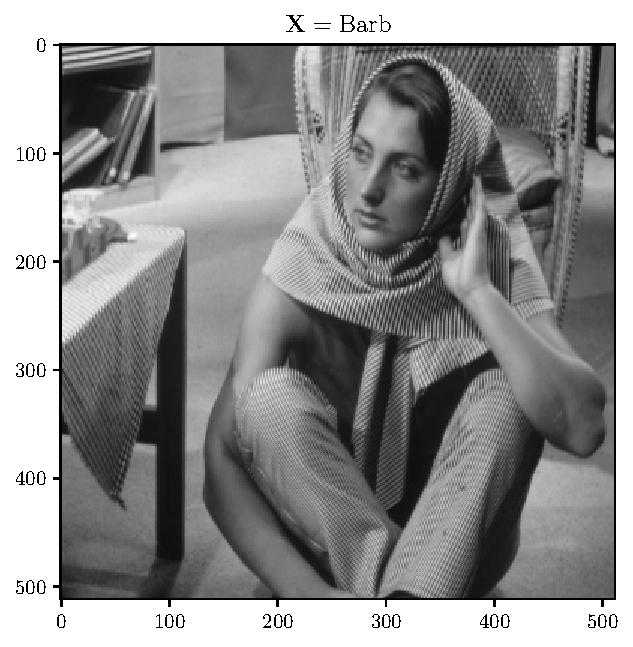
\includegraphics{barb.pdf}} & \href{https://nbviewer.org/github/vicente-gonzalez-ruiz/denoising/blob/main/notebooks/barb_0MMPG.ipynb\#barb_0MMPG}{\includegraphics{barb_0MMPG.pdf}} \\
      \href{https://nbviewer.org/github/vicente-gonzalez-ruiz/denoising/blob/main/notebooks/barb_averaging.ipynb\#barb_averaging}{\includegraphics{barb_averaging.pdf}} & \href{https://nbviewer.org/github/vicente-gonzalez-ruiz/denoising/blob/main/notebooks/barb_averaging_PSNR.ipynb\#barb_averaging_PSNR}{\includegraphics{barb_averaging_PSNR.pdf}}
    \end{tabular}
  }
  \caption{Increase of the SNR as a function of the number of noisy
    instances used in MNI. The clean image is shown on the top-left,
    and a noisy instance on the top-right. On the bottom-left, the
    denoised NMI image, and on the bottom-right the progression of the
    SNR as a function of $I$ and the level of
    noise.\label{fig:MNI_0MMPG}}
\end{figure}

\begin{comment}
%{{{

Fig.~\ref{fig:0MAUN} shows an
example of how zero-mean uniform noise is cancelled by averaging.
  
  \begin{figure}
    \centering
    \resizebox{1.0\textwidth}{!}{
      \renewcommand{\arraystretch}{0.0} % Adjust row spacing in the table
      \setlength{\tabcolsep}{0ex}      % Adjust column spacing in the table    
      \begin{tabular}{cc}
        \href{https://nbviewer.org/github/vicente-gonzalez-ruiz/denoising/blob/main/figs/averaging_denoising.ipynb\#Display-Barb}{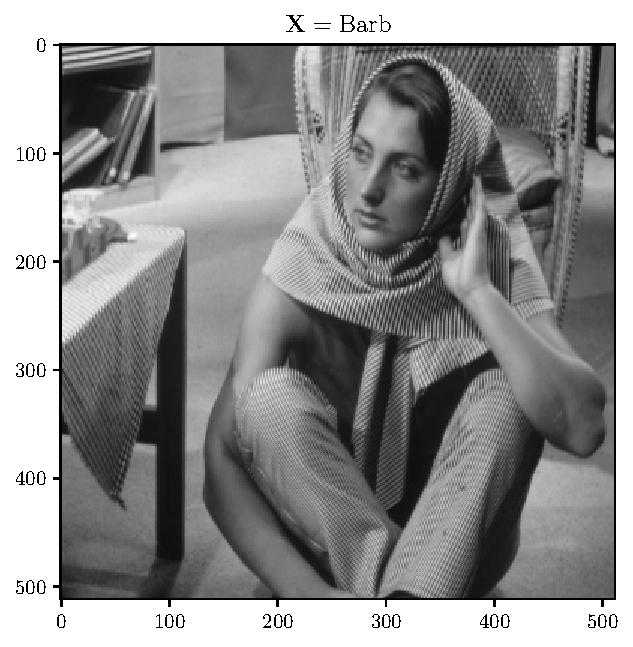
\includegraphics{barb}} & \href{https://nbviewer.org/github/vicente-gonzalez-ruiz/denoising/blob/main/figs/averaging_denoising.ipynb\#0MAUN_barb}{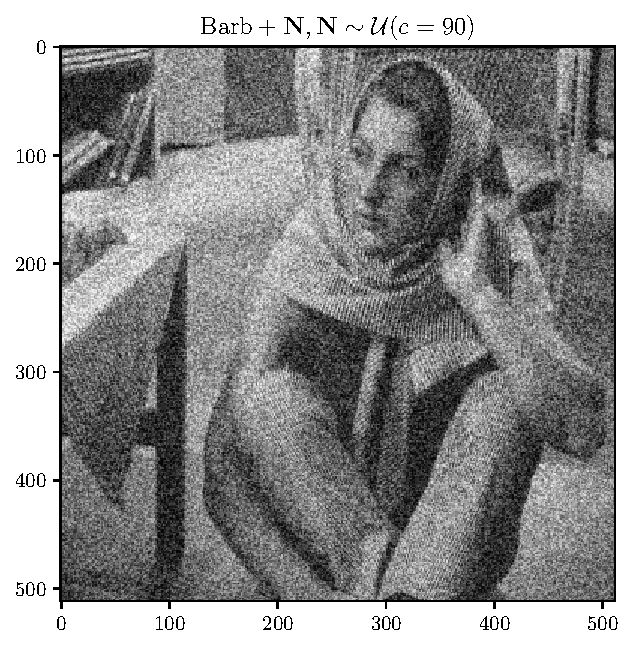
\includegraphics{0MAUN_barb}} \\
        \href{https://nbviewer.org/github/vicente-gonzalez-ruiz/denoising/blob/main/figs/averaging_denoising.ipynb\#denoised_0MAUN_barb}{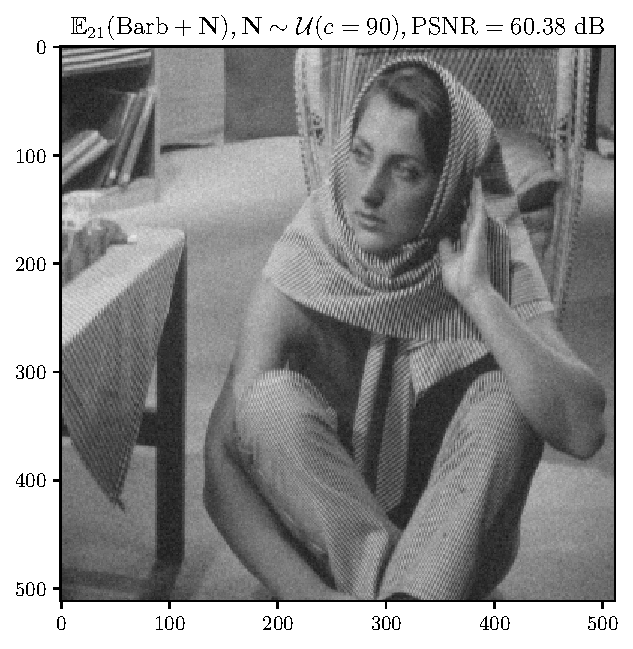
\includegraphics{denoised_0MAUN_barb}} & \href{https://nbviewer.org/github/vicente-gonzalez-ruiz/denoising/blob/main/figs/averaging_denoising.ipynb\#PSNR_0MAUN_barb}{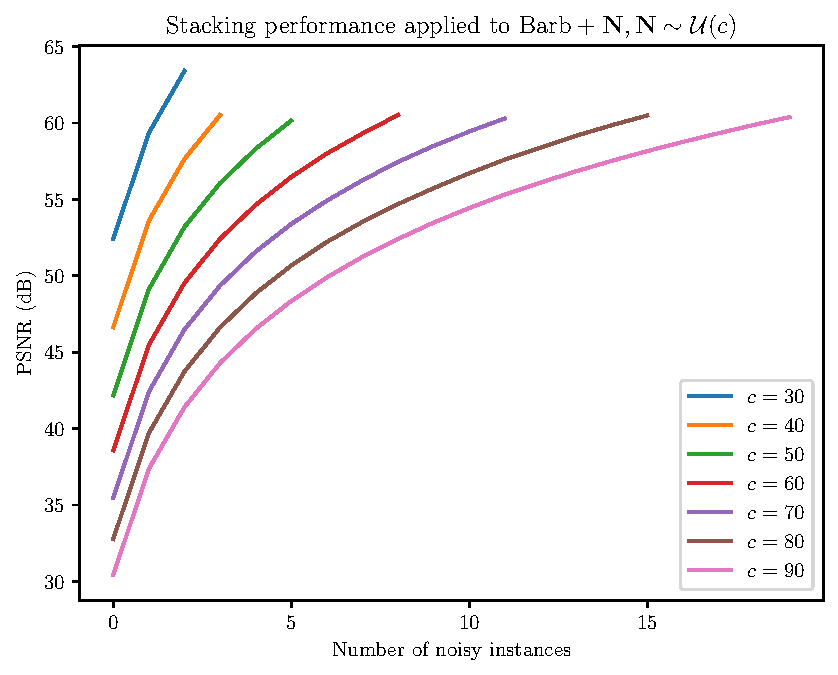
\includegraphics{PSNR_0MAUN_barb}}
      \end{tabular}
    }
    \caption{Effect of zero-mean additive uniform noise in an image
      and how averaging can be used to reduced by averaging. The clean
      image of Barb is shown on the top left, and a noisy version on
      the top right. On to bottom, the left image shows a denoised
      version after averaging and the right graph shows the performance
      of the averaging process for different levels of
      noise.\label{fig:0MAUN}}
  \end{figure}

 Fig.~\ref{fig:0MAGN} shows an
  example of how zero-mean Gaussian noise is cancelled by averaging.

  \begin{figure}
    \centering
    \resizebox{1.0\textwidth}{!}{
      \renewcommand{\arraystretch}{0.0} % Adjust row spacing in the table
      \setlength{\tabcolsep}{0ex}      % Adjust column spacing in the table    
      \begin{tabular}{cc}
        \href{https://nbviewer.org/github/vicente-gonzalez-ruiz/denoising/blob/main/figs/averaging_denoising.ipynb\#barb}{\includegraphics{barb}} & \href{https://nbviewer.org/github/vicente-gonzalez-ruiz/denoising/blob/main/figs/averaging_denoising.ipynb\#0MAGN_barb}{\includegraphics{0MAGN_barb}} \\
        \href{https://nbviewer.org/github/vicente-gonzalez-ruiz/denoising/blob/main/figs/averaging_denoising.ipynb\#denoised_0MAGN_barb}{\includegraphics{denoised_0MAGN_barb}} & \href{https://nbviewer.org/github/vicente-gonzalez-ruiz/denoising/blob/main/figs/averaging_denoising.ipynb\#PSNR_0MAGN_barb}{\includegraphics{PSNR_0MAGN_barb}}
      \end{tabular}
    }
    \caption{Effect of zero-mean additive Gaussian noise in an image
      and how averaging can be used to reduced by averaging. The clean
      image of Barb is shown on the top left, and a noisy version on
      the top right. On to bottom, the left image shows a denoised
      version after averaging and the right graph shows the performance
      of the averaging process for different levels of
      noise.\label{fig:0MAGN}}
  \end{figure}

  Fig.~\ref{fig:0MMGN} shows an example of
  how zero-mean Gaussian noise is cancelled by averaging.

  \begin{figure}
    \centering
    \resizebox{1.0\textwidth}{!}{
      \renewcommand{\arraystretch}{0.0} % Adjust row spacing in the table
      \setlength{\tabcolsep}{0ex}      % Adjust column spacing in the table    
      \begin{tabular}{cc}
        \href{https://nbviewer.org/github/vicente-gonzalez-ruiz/denoising/blob/main/figs/averaging_denoising.ipynb\#barb}{\includegraphics{barb}} & \href{https://nbviewer.org/github/vicente-gonzalez-ruiz/denoising/blob/main/figs/averaging_denoising.ipynb\#0MMGN_barb}{\includegraphics{0MMGN_barb}} \\
        \href{https://nbviewer.org/github/vicente-gonzalez-ruiz/denoising/blob/main/figs/averaging_denoising.ipynb\#denoised_0MMGN_barb}{\includegraphics{denoised_0MMGN_barb}} & \href{https://nbviewer.org/github/vicente-gonzalez-ruiz/denoising/blob/main/figs/averaging_denoising.ipynb\#PSNR_0MMGN_barb}{\includegraphics{PSNR_0MMGN_barb}}
      \end{tabular}
    }
    \caption{Effect of zero-mean multiplicative Gaussian noise in an
      image and how averaging can be used to reduced by averaging. The
      clean image of Barb is shown on the top left, and a noisy
      version on the top right. On to bottom, the left image shows a
      denoised version after averaging and the right graph shows the
      performance of the averaging process for different levels of
      noise.\label{fig:0MMGN}}
  \end{figure}

 Fig.~\ref{fig:Rayleigh}
  shows an example of how Rayleigh noise is cancelled by averaging.

  \begin{figure}
    \centering
    \resizebox{1.0\textwidth}{!}{
      \renewcommand{\arraystretch}{0.0} % Adjust row spacing in the table
      \setlength{\tabcolsep}{0ex}      % Adjust column spacing in the table    
      \begin{tabular}{cc}
        \href{https://nbviewer.org/github/vicente-gonzalez-ruiz/denoising/blob/main/figs/averaging_denoising.ipynb\#barb}{\includegraphics{barb}} & \href{https://nbviewer.org/github/vicente-gonzalez-ruiz/denoising/blob/main/figs/averaging_denoising.ipynb\#Rayleigh_barb}{\includegraphics{Rayleigh_barb}} \\
        \href{https://nbviewer.org/github/vicente-gonzalez-ruiz/denoising/blob/main/figs/averaging_denoising.ipynb\#denoised_Rayleigh_barb}{\includegraphics{denoised_Rayleigh_barb}} & \href{https://nbviewer.org/github/vicente-gonzalez-ruiz/denoising/blob/main/figs/averaging_denoising.ipynb\#PSNR_Rayleigh_barb}{\includegraphics{PSNR_Rayleigh_barb}}
      \end{tabular}
    }
    \caption{Effect of Rayleigh noise in an image and how averaging can
      be used to reduced by averaging. The clean image of Barb is shown
      on the top left, and a noisy version on the top right. On to
      bottom, the left image shows a denoised version after averaging
      and the right graph shows the performance of the averaging
      process for different levels of noise.\label{fig:Rayleigh}}
  \end{figure}

  Fig.~\ref{fig:Poisson} shows an example of how Poisson noise is
  cancelled by averaging.

  \begin{figure}
    \centering
    \resizebox{1.0\textwidth}{!}{
      \renewcommand{\arraystretch}{0.0} % Adjust row spacing in the table
      \setlength{\tabcolsep}{0ex}      % Adjust column spacing in the table    
      \begin{tabular}{cc}
        \href{https://nbviewer.org/github/vicente-gonzalez-ruiz/denoising/blob/main/figs/averaging_denoising.ipynb\#barb}{\includegraphics{barb}} & \href{https://nbviewer.org/github/vicente-gonzalez-ruiz/denoising/blob/main/figs/averaging_denoising.ipynb\#Poisson_barb}{\includegraphics{Poisson_barb}} \\
        \href{https://nbviewer.org/github/vicente-gonzalez-ruiz/denoising/blob/main/figs/averaging_denoising.ipynb\#denoised_Poisson_barb}{\includegraphics{denoised_Poisson_barb}} & \href{https://nbviewer.org/github/vicente-gonzalez-ruiz/denoising/blob/main/figs/averaging_denoising.ipynb\#PSNR_Poisson_barb}{\includegraphics{PSNR_Poisson_barb}}
      \end{tabular}
    }
    \caption{Effect of Poisson noise in an image and how averaging can
      be used to reduced by averaging. The clean image is shown
      on the top left, and a noisy version on the top right. On the
      bottom, the left image shows a denoised version after averaging
      and the right graph shows the performance of the averaging
      process for different levels of noise.\label{fig:Poisson}}
  \end{figure}

%}}}
\end{comment}

%}}}

\subsection{Gaussian Filtering (GF)}
%{{{

Gaussian noising is based on the use of low-pass
(smoothing)\footnote{Because random noise typically consists of sharp
  transitions in intensity, an obvious application of smoothing is
  noise reduction \cite{gonzalez1992digital}.} Gaussian
filters. Unlike other digital filters, such as an ideal low-pass
filter, a Gaussian low-pass filter does not generate ringing (the
transfer function of a Gaussian filter is another Gaussian filter,
which has not lobes), and the convolution of two Gaussians are Gaussian
functions also. 

In GF denoising, a 1D Gaussian kernel $\mathbf{h}$ is convolved with
the noisy instance $\hat{\mathbf{X}}$ to obtain
\begin{equation}
  \tilde{\mathbf{X}} = \hat{\mathbf{X}}*\mathbf{h},
  \label{eq:GF}
\end{equation}
where $\tilde{\mathbf{X}}$ represents the denoised signal, and $*$ the
convolution between digital signals. As can be seen, unlike MNI, GF
requires only one instance.

The coefficients of $\mathbf{h}$ define a low-pass\footnote{We can
  distinguish this because all are positive coefficients.}
filter, which are sampled from
\begin{equation}
  h(x) = \frac{1}{\sqrt{2\pi}\tau}e^{-\frac{{x}^2}{(2\tau^2)}},
  \label{eq:GK}
\end{equation}
where $x$ represents a distance in
the signal domain, and $\tau$ (known as the \emph{standard deviation}
\footnote{Notice that the filter coefficients are also the values that a
  discrete random variable takes from a normal distribution.})
determines the bandwidth of the filter.

\begin{figure}
  \centering
  \includegraphics[width=0.8\textwidth]{3D_GF}
  \caption{3D Gaussian filtering. The gray planes contain the voxels
    that are filtered and the white planes contain the voxels used by
    the 1D kernel when it is applied to the voxels of the filtered
    plane. The kernel shown here contains 3 coefficients. The volume
    is convolved sequentially in-place, from left to
    right.\label{fig:3D_GF}}
\end{figure}

Multidimensional GF is separable (see
Appendix~\ref{ape:GF_separability}), which means that we can apply the
1D filter to the $D$ dimensions of the signal to compute a $D$D
denoising. De facto, Gaussian kernels are the only circularly
symmetric kernels that are also separable
\cite{gonzalez1992digital}. For the 3D case (see
Fig.~\ref{fig:3D_GF}), we have that
\begin{equation}
  \tilde{\mathbf{X}} = \Big(\big(\hat{\mathbf X}*^{(\text{Z})}{\mathbf h}\big)*^{(\text{Y})}{\mathbf h}\Big)*^{(\text{X})}{\mathbf h},
    \label{eq:3D_GF}
\end{equation}
where ${\mathbf s}*^{(d)}{\mathbf h}$ is the 1D convolution applied to
the dimension $d$ of the signal ${\mathbf s}$ and the (1D) kernel
${\mathbf h}$. For simplicity, Eq.~\ref{eq:3D_GF} defines isotropic
filtering, but $\tau$ can be different at each dimension to provide
anisotropy. Eq.~\ref{eq:3D_GF} is implemented
\href{https://github.com/vicente-gonzalez-ruiz/denoising/blob/main/src/denoising/volume/gaussian.py}{here},
and the corresponding 2D version is implemented
\href{https://github.com/vicente-gonzalez-ruiz/denoising/blob/main/src/denoising/image/gaussian.py}{here}.

\begin{comment}
%{{{

 This idea has been describen in Python pseudo-code in
the Fig.~\ref{fig:3DGF_imple}.

\begin{figure}
\noindent $\mathsf{3DGF}(\hat{\mathbf{X}}, \mathbf{h})$: $\rightarrow\tilde{\mathbf{X}}$
\vspace{-1ex}
\begin{enumerate}
  \setlength{\itemsep}{0pt}
\item [1.] $\tilde{\mathbf{X}}\leftarrow\href{https://docs.opencv.org/2.4/modules/imgproc/doc/geometric_transformations.html#resize}{\mathsf{resize}}(\hat{\mathbf{X}}, \mathsf{dsize}=)$
\item [2.] $\mathsf{for}~z~\mathsf{in}~\mathsf{range}(\hat{\textbf{X}}.\mathsf{shape}_0),~\mathsf{run}$:  \hfill $\mathtt{/*~Filtering~in~the~Z~direction~*/}$
  \begin{enumerate}
  \item [1.] $\mathsf{for}~h~\mathsf{in~range}(\mathbf{h}.\mathsf{size})$:
    \begin{enumerate}
    \item [1.] $\tilde{\mathbf{X}}_{z,:,:}\leftarrow\tilde{\mathbf{X}}_{z,:,:}+\hat{\mathbf{X}}_{z,:,:}\mathbf{h}_{h}$
    \end{enumerate}
  \end{enumerate}
\item [3.] $\mathsf{for}~y~\mathsf{in}~\mathsf{range}(\hat{\textbf{X}}.\mathsf{shape}_1),~\mathsf{run}$:  \hfill $\mathtt{/*~Filtering~in~the~Y~direction~*/}$
  \begin{enumerate}
  \item [1.] $\mathsf{for}~k~\mathsf{in~range}(\mathbf{h}.\mathsf{size})$:
    \begin{enumerate}
    \item [1.] $\tilde{\mathbf{X}}_{:,y,:}\leftarrow\tilde{\mathbf{X}}_{:,y,:}+\hat{\mathbf{X}}_{:,y,:}\mathbf{h}_{h}$
    \end{enumerate}
  \end{enumerate}
\item [4.] $\mathsf{for}~x~\mathsf{in}~\mathsf{range}(\hat{\textbf{X}}.\mathsf{shape}_2),~\mathsf{run}$:  \hfill $\mathtt{/*~Filtering~in~the~X~direction~*/}$
  \begin{enumerate}
  \item [1.] $\mathsf{for}~h~\mathsf{in~range}(\mathbf{h}.\mathsf{size})$:
    \begin{enumerate}
    \item [1.] $\tilde{\mathbf{X}}_{:,:,x}\leftarrow\tilde{\mathbf{X}}_{:,:,x}+\hat{\mathbf{X}}_{:,:,x}\mathbf{h}_{h}$
    \end{enumerate}
  \end{enumerate}
\end{enumerate}
%\end{myquote}
\caption{Python pseudo-code of 3DGF using periodic signal extension.}
\label{fig:3DGF_imple}
\end{figure}

%}}}
\end{comment}

\begin{figure}
  \centering
  \resizebox{1.0\textwidth}{!}{
    \renewcommand{\arraystretch}{0.0} % Adjust row spacing in the table
    \setlength{\tabcolsep}{0ex}      % Adjust column spacing in the table    
    \begin{tabular}{cc}
      %\href{https://nbviewer.org/github/vicente-gonzalez-ruiz/denoising/blob/main/notebooks/barb.ipynb}{\includegraphics{barb}} & \href{https://nbviewer.org/github/vicente-gonzalez-ruiz/denoising/blob/main/figs/lake.ipynb}{\includegraphics{lake}} \\
      %\href{https://nbviewer.org/github/vicente-gonzalez-ruiz/denoising/blob/main/notebooks/barb_0MMPG.ipynb}{\includegraphics{barb_0MMPG}} & \href{https://nbviewer.org/github/vicente-gonzalez-ruiz/denoising/blob/main/notebooks/lake_0MMPG.ipynb}{\includegraphics{lake_0MMPG}} \\
      \href{https://nbviewer.org/github/vicente-gonzalez-ruiz/denoising/blob/main/notebooks/Confocal_FISH_GF_optimal_tau.ipynb\#Confocal_FISH_GF_optimal_tau}{\includegraphics{Confocal_FISH_GF_optimal_tau.pdf}} & \href{https://nbviewer.org/github/vicente-gonzalez-ruiz/denoising/blob/main/notebooks/TwoPhoton_MICE_GF_optimal_tau.ipynb\#TwoPhoton_MICE_GF_optimal_tau}{\includegraphics{TwoPhoton_MICE_GF_optimal_tau.pdf}}
    \end{tabular}
  }
  \caption{Optimal $\tau$ values in GF.\label{fig:optimal_GF_tau}}
\end{figure}

As can be seen in Eq.~\ref{eq:GK}, the denoising result depends on
$\tau$. An optimal value for the standard deviation, $\tau^*$, can be
found if we know $\mathbf{X}$ (see
Fig.~\ref{fig:optimal_GF_tau}). Unfortunately, $\mathbf{X}$ is usually
unknown and we only can estimate $\tau^*$. Ideally, $\tau^*$ should
increase the SNR as much as possible, considering also that: (1) GF
attenuates the high frequencies, (2) the SFC of the noise is close to
zero, and (3) that most of the energy (information) in the signals are
concentrated in the low frequencies. Therefore, we should find a
cut-off frequency
\begin{equation}
  \eta^* = \text{min}\{\eta|\text{SFC}(\hat{\mathbf{X}})_\eta < \alpha\},
  \label{eq:search_eta}
\end{equation}
where $\alpha$ is the minimun correlation that should reach the SFC to consider that the corresponding ring/shell has a high enough SNR (see
Appendix~\ref{ape:tau_VS_eta}). Once we have already estimated
$\eta^*$, we can use the corresponding $\tau^*$ to filter out those
frequency components of $\hat{\mathbf{X}}$ with the lowest SNR.

\begin{figure}
  \centering
  \resizebox{1.0\textwidth}{!}{
    \renewcommand{\arraystretch}{0.0} % Adjust row spacing in the table
    \setlength{\tabcolsep}{0ex}      % Adjust column spacing in the table    
    \begin{tabular}{cc}
      \href{https://nbviewer.org/github/vicente-gonzalez-ruiz/denoising/blob/main/notebooks/Confocal_FISH_GF_estimation.ipynb}{\includegraphics{Confocal_FISH_GF_estimation.pdf}} & \href{https://nbviewer.org/github/vicente-gonzalez-ruiz/denoising/blob/main/notebooks/TwoPhoton_MICE_GF_estimation.ipynb}{\includegraphics{TwoPhoton_MICE_GF_estimation.pdf}}
    \end{tabular}
  }
  \caption{Optimal VS estimated $\tau^*$ values.\label{fig:tau_GF_estimation}}
\end{figure}

In the Fig.~\ref{fig:tau_GF_estimation} there is a comparison between
the true $\tau^*$ values and their estimations, using the EOS
technique (see Appendix~\ref{ape:EOS}) to compute the SFC curves (see
Section~\ref{sec:fourier_correlation}). Specifically, we have used
(see Eq.~\ref{eq:ideal_hat_tau} and Fig.~\ref{fig:eta_vs_tau})
\begin{equation}
  \tau^*_{\text{EOS}} = \frac{0.141}{2\eta^*},
  \label{eq:tau_VS_eta_empirical_EOS}
\end{equation}
(and not exactly the fitting expression shown in the
Fig.~\ref{fig:gaussian_leakage}) because using signal splitting to
compute the SFC, only the first half of the frequencies provide
reliable information. Notice that, to determine $\eta^*$ (the
estimated ``optimal'' cut-off frequency of the Gaussian filter) we
have assumed that an attenuation higher than $1/\sqrt{2}$ (see
Appendix~\ref{ape:tau_VS_eta}) can be high enought to filter out the
frequencies higher than $\eta^*$.

Appendix~\ref{ape:results} contains a table with the performance of
some denoisers.

%{\color{red} Podemos comparar diferentes algoritmos de denoising si usamos, para una determinada configuración de ruido, el filtrado óptimo (que es posible encontrar porque tenemos el GT). Nos va a salir una tabla con valores de PCC.}

%Since all denoising algorithms have a similar behavior (they tend to
%eliminate high frequencies and preserve low ones), we will consider
%Eq.~\ref{eq:tau_VS_eta_empirical_EOS} as generic and it will be used
%to find the optimal value of the different operating parameters of the
%denoising algorithms.

\begin{comment}
%{{{

Concretelly, we use (see
Appendix~\ref{SFC_random_data})
\begin{equation}
  \tau^*_{\text{SPRS}} = \frac{0.141}{5(\eta^*-0.09)},
  \label{eq:tau_VS_eta_empirical_SPRS}
\end{equation}
when we are using the SPRS algorithm to find the SFC curve, or
\begin{equation}
  \tau^*_{\text{EO}} = \frac{0.141}{3(\eta^*-0.01)},
  \label{eq:tau_VS_eta_empirical_EO}
\end{equation}
if we are using the EO algorithm to find the SFC curve,
where we are supposing that $\beta=1/\sqrt{2}$ (see
Appendix~\ref{ape:tau_VS_eta}). 

Fig.~\ref{fig:tau_GF_estimation} shows the result of using
Eqs.~\ref{eq:tau_VS_eta_empirical_SPRS} and
\ref{eq:tau_VS_eta_empirical_EO} for estimating $\tau^*$ for the two
test images. As can be seen ..

%}}}
\end{comment}

\begin{comment}
%{{{

Assuming that most of the signal energy (information) is concentrated
in the low frequencies, higher values of $\tau$ will produce a higher
smoothing effect in $\tilde{\mathbf{X}}$). More concretely, if
$\mathcal{F}(h)=H$, that is
\begin{equation}
  H(u) = e^{-\frac{u^2}{2\tau^{-2}}},
\end{equation}
it can be seen that if $\tau$ increases, the cut-off frequency
provided by $H$ decreases, and viceversa. 


\begin{figure}
  \centering
  \resizebox{1.0\textwidth}{!}{
    \renewcommand{\arraystretch}{0.0} % Adjust row spacing in the table
    \setlength{\tabcolsep}{0ex}      % Adjust column spacing in the table    
    \begin{tabular}{cc}
      \href{https://nbviewer.org/github/vicente-gonzalez-ruiz/denoising/blob/main/notebooks/barb.ipynb}{\includegraphics{barb}} & \href{https://nbviewer.org/github/vicente-gonzalez-ruiz/denoising/blob/main/figs/lake.ipynb}{\includegraphics{lake}} \\
      \href{https://nbviewer.org/github/vicente-gonzalez-ruiz/denoising/blob/main/notebooks/tau_VS_img.ipynb\#0MMPG_barb}{\includegraphics{0MMPG_barb}} & \href{https://nbviewer.org/github/vicente-gonzalez-ruiz/denoising/blob/main/figs/tau_VS_img.ipynb\#0MMPG_lake}{\includegraphics{0MMPG_lake}} \\
      \href{https://nbviewer.org/github/vicente-gonzalez-ruiz/denoising/blob/main/notebooks/tau_VS_img.ipynb\#GF_0MMPG_barb}{\includegraphics{GF_0MMPG_barb}} & \href{https://nbviewer.org/github/vicente-gonzalez-ruiz/denoising/blob/main/figs/tau_VS_img.ipynb\#GF_0MMPG_lake}{\includegraphics{GF_0MMPG_lake}}
    \end{tabular}
  }
  \caption{Two examples of optimal denoising using GF. On the top, the
    original images. In the middle, the noisy instances. On the
    bottom, the denoised images. {\color{red} arreglar PSNRs y elegir
      tau optimo para ejemplo}\label{fig:GF_tau_optimal}}
\end{figure}

Fig.~\ref{fig:tau_VS_image} shows the denoising performance of GF for
two artificially noised images, for different levels of noise
($\sigma$) and filter length ($\tau$). As can be seen, the optimal
value of the filter length, $\tau^*$ (which maximizes the PCC between
$\mathbf{X}$ and $\tilde{\mathbf{X}}$), depends on the noise level and
$\mathbf{X}$, information that is, in general, unavailable in
microscopy imaging. Therefore, $\tau^*$ can be only
\emph{estimated}\footnote{Notice that, only knowing $\mathbf{X}$ it
  would be possible to find $\tau^*$. Therefore, the furthest one can
  go is to estimate the optimal filtering parameters}. depending on,
for example, the (subjective) visual quality of
$\tilde{\mathbf{X}}$. An example of optimal denoising using GF has
been show in Fig.~\ref{fig:GF_tau_optimal}.

% \begin{figure}
%   \centering
%   \resizebox{1.0\textwidth}{!}{
%     \renewcommand{\arraystretch}{0.0} % Adjust row spacing in the table
%     \setlength{\tabcolsep}{0ex}      % Adjust column spacing in the table    
%     \begin{tabular}{cc}
%   \href{https://nbviewer.org/github/vicente-gonzalez-ruiz/denoising/blob/main/figs/gaussian_denoising.ipynb\#GD_SFRC_0MMPG_NL20_barb}{\includegraphics{GD_SFRC_0MMPG_NL20_barb}} & \href{https://nbviewer.org/github/vicente-gonzalez-ruiz/denoising/blob/main/figs/gaussian_denoising.ipynb\#GD_SFRC_0MMPG_NL60_barb}{\includegraphics{GD_SFRC_0MMPG_NL60_barb}}
%     \end{tabular}
%     }
%     \caption{SFRC curves for two different noisy instances of
%       Barb, see Fig.~\ref{fig:tau_VS_image} using two
%       different noise levels ($\sigma=20$ and $\sigma=60$), and after
%       having applied GD for several filter lengths. As can be seen, for $\sigma=20$, the ``optimal'' filter
%       length (that maximizes the area below the curve) is ..., and for
%       $\sigma=60$, the ``optimal'' filter length is ... Therefore, the
%       ``optimal'' filter length is (positively) correlated with the
%       noise level. Notice that $\tau$
%       has been discretized in steps of $0.25$.

%       (2) the
%       ``optimal'' filter length is (positively) correlated with the
%       noise level (for the noise level $\sigma=40$ and $\gamma=0.15$
%       the ``optimal'' $\tau=1.0$ and the noise level $\sigma=50$ and
%       $\gamma=0.15$ the ``optimal'' $\tau=1.25$). Notice that $\tau$
%       has been discretized in steps of $0.25$.


%       Relation between the SFRC curves and the filter length of
%       a Gaussian filter. $\hat{\mathbf{X}}_1$ is the the noise image
%       (Barb) shown in the Fig.~\ref{fig:tau_VS_image} (for $\sigma=40$
%       and $\gamma=0.15$). As can be seen, the area below the curve is
%       maximized for $\tau=1.0$

%       Effect of zero-mean MPG noise in an image and how GD
%     can be used to reduce it. A noisy version of the
%     image is on the top-left. On the top-right, the SFRC curves
%     of the denoised image for different filter lengths. As can be seen
%     in this subfigure, for the noise level
%     $(\sigma=40, \gamma=0.15)$, an optimal $\tau=1.25$ should be used if
%     (considering that the area below the SFRC curve should be maximized).
%     On the bottom-left, it can be seen that for this noise level,
%     the ``optimal'' Gaussian kernel-lenght is $\tau/2=0.625 \approx 0.7$. The resulting
%     ``optimal'' filtered image (using GD) is shown on the bottom-right.
%     \label{fig:GD_0MMPG}}
% \end{figure}

{\color{red} ------ comienzo sin terminar ------ }

It is also possible to estimate $\tau^*$ using the self-correlation in
the Fourier domain \cite{koho2019fourier} {\color{red}Este sería un
  buen punto para hablar de cómo estamos calculando la curva
  SF{R|S}C}. The idea here is to determine the frequency $u^*$ for
which, to the right of this frequency, the SNR decays under some given
threshold.

A more objective procedure to estimate $\tau^*$ should be based on
some (objective) quality metric, such as the self-correlation in the
Fourier domain \cite{koho2019fourier}. Fig.~\ref{fig:GD_0MMPG} shows
the result of using the SFRC of the noisy image to estimate $\tau^*$,
considering the idea that the low-pass filter should remove those
frequency components where the SNR is lower than a given threshold.



Fig.~\ref{fig:GD_0MMPG} shows
SFRC curves for different filter lengths, and it has been also
computed the normalized area below each curve, a metric that is
(positively) correlated with $\tau^*$ (see
Fig.~\ref{fig:tau_VS_image}). As can be seen that, $\tau^*$ can be
estimated using the filter length that maximizes the area below the
corresponding SFRC curve.


because the
higher the area, the higher also the PCC between the Fourier
coefficients


and it can be seen, the normalized area below the curve can be used to estimate


Another alternative can use some heuristic to estimate

We propose a more automatic procedure to find $\tau^*$.  by maximizing
the ratio between the amount of noise and the amount of signal removed
by the filter. To determine this, we can use the SFRC curve (see
Sec.~\ref{sec:FSC}), in which each point represents the correlation
between two\footnote{Actually, each point is the average (arithmetic
  mean) of two correlation coefficients, each one obtained after
  subsampling the image in each dimension (by rows, and by columns).}
rings of Fourier coefficients, extracted from two subsampled versions
of $\tilde{\mathbf{X}}$.

for the single parameter that GD requires (the length of
the Gaussian kernels in each dimension, represented by $\tau$ in
$\mathrm{GD}_\tau$) depends on the noise level, an information that is
generally unknown in microscopy imaging.

To estimate the relation between the filter length that should
maximize the quality of the denoised signal, the SFRC (Self Fourier
Ring Correlation, see Section~\ref{sec:FSC}) of several noisy
instances of the same image (variying the level of noise) has been
shown in the Fig.~\ref{fig:SFRC}.

has been calculated by subbands of a filtered
image, generating a number of SFRC curves, one for each different
kernel length $\tau$ (see Fig.  \ref{fig:GD_0MMPG}). As can be seen,
the autocorrelation increases when the noise level decreases due to
increasing $\tau$, until it reaches a value for which the
autocorrelation decreases again\footnote{Remember that the SFRC metric
  quantifies the correlation between subsampled versions of the same
  input signal and that, by definition, the MPG noise should be
  uncorrelated. For this reason, if noise were only had at the input,
  we should obtain a flat SFRC that approximates to zero. Therefore,
  the higher the area below the SFRC curve, the higher the presence of
  signal.}. For that $\tau^*$, which maximizes the area under the
curve up to the normalized frequency $\omega/4$, is when the PCC
metric is also maximized (considering the original image resolution,
i.e., without the subsampling required to compute the SFRC) for
$\tau^*/2$, which means that we can use the SFRC metric (in the 2D
case) and the SFSC (in the 3D case) to estimate the optimal filtering
parameters knowing only the noisy instance $\hat{\mathbf{X}}$.

{\color{red} ------ fin sin terminar ------ }

%}}}
\end{comment}

%}}}

%  \section{Beltrami flow}
% Parece que se usa en AND, pero no se bien cómo.

%\section{Median filter}

%\section{Bilateral filter}

\subsection{Wiener Filtering (WF)}
The Wiener filter \cite{wiener1942extrapolation} is an adaptive linear
filter designed to minimize the MSE between the denoised signal
$\tilde{\mathbf{x}}$ and clean signal $\mathbf{x}$, when this has been
corrupted\footnote{A Wiener filter also considers that $\mathbf{x}$
  can be affected, apart from the noise, by some linear transformation
  (such as a blurring), but we will ingnore this.} by noise. For this
reason, WF is also known by \emph{minimum MSE filtering} and also by
\emph{least square error fitering}. When the filter is used only for
removing noise, we are refering to denoising.

To use WF, the next conditions must be satisfied:
\begin{enumerate}
\item The noise is not correlated with the original signal, i.e., the
  noise is ZAWG.
\item The mean of the noise is zero.
\item Signal and noise are stationary random processes (their mean and
  variance remains constant).
\end{enumerate}

Under these assumptions, WF minimizes the MSE between the output of
the filter $\tilde{\mathbf{x}}$ (the filtered signal) and the
(unknown) clean signal $\mathbf{x}$,
\begin{equation}
  \mathbb{E}[(\tilde{\mathbf{x}} - \mathbf{x})^2].
  \label{eq:WF_objective}
\end{equation}
Because $\mathbf{x}$ is seldom known, the WF uses the statistics of
$\hat{\mathbf{x}}$ (the noisy signal) to approximate to
Eq.~\ref{eq:WF_objective} (in other words, in general we can only
estimate $\tilde{\mathbf{x}}$). It can be demostrated that such
estimation can be found as \cite{wiener1942extrapolation}
\begin{equation}
  \tilde{\mathbf{x}} = \text{DFT}^{-1}(\hat{\mathbf{X}}\mathbf{H}),
\end{equation}
where $\hat{\mathbf{X}}$ is the DFT of $\hat{\mathbf{x}}$, and
\begin{equation}
  \mathbf{H} = \frac{\text{PSD}(\hat{\mathbf{x}})}{\text{PSD}(\hat{\mathbf{x}}) + \text{PSD}(\mathbf{n})}
  \label{eq:WF_frequency_response}
\end{equation}
is the frequency response of the Wiener filter (its transfer
function). If the noise is ZAWF, the PSD can be approximated by the
variance in a. Therefore, Eq.~\ref{eq:WF_frequency_response} becomes
\begin{equation}
  \mathbf{H}_k = \frac{\mathbb{V}(\hat{\mathbf{X}}_k)}{\mathbb{V}(\hat{\mathbf{X}}_k) + \sigma^2_{\mathbf{n}}},
  \label{eq:WF_coeffs}
\end{equation}
where $\mathbb{V}(\hat{\mathbf{X}}_k)$ is the variance of the $k$-th
Fourier coefficient of the $\text{DFT}(\hat{\mathbf{x}})$ over a
collection of $\hat{\mathbf{x}}$ instances, and $\sigma^2_{\mathbf{n}}$ is (an
estimation of) the variance of the noise. For this reason, the signal
is typically processed by blocks. For example, the
implementation offered in Scipy
(\href{https://docs.scipy.org/doc/scipy/reference/generated/scipy.signal.wiener.html}{\texttt{scipy.signal.wiener}})
requires two arguments:
\begin{enumerate}
\item The noise power, expressed as the average variance of the noise
  which by default is
  ${\sigma^2_{\mathbf{n}}}=
  \mathbb{E}\left(\mathbb{V}(\hat{\mathbf{x}})\right)$. If the GT
  signal were known, the noise power\footnote{Remember that the noise
    isuncorrelated with the GT signal, and therefore the power of the
    noise is the same in all the windows, on average.} can be found as
  \begin{equation}
    {\sigma^2}^*_{\mathbf{n}} = \mathbb{E}\left(\mathbb{V}(\hat{\mathbf{x}}-\mathbf{x})\right).
  \end{equation}
\item The window size $w$, which is the side of the (usually square)
  window of pixels $\hat{\mathbf{x}}_{[i]}$ (a window with side $w$
  centered at the $i$-th sample of the noisy signal). In general,
  because $\sigma^2_{\mathbf{n}}$ is unknown, the denoising process
  should be controlled using $w$ (the larger $w$, the greater the
  filtering effect).
\end{enumerate}
Concretelly,
\begin{equation}
  \tilde{\mathbf{x}}_i = \left\{
    \begin{array}{ll}
      \mathbb{E}(\hat{\mathbf{x}}_{[i]}) + \frac{\mathbb{V}(\hat{\mathbf{x}}_{[i]})-\sigma^2_\mathbf{n}}{\mathbb{V}(\hat{\mathbf{x}}_{[i]})}\left(\hat{\mathbf{x}}_i-\mathbb{E}(\hat{\mathbf{x}}_{[i]})\right) & : \ \mathbb{V}(\hat{\mathbf{x}}_{i]}) < \sigma^2_\mathbf{n} \\
\mathbb{E}(\hat{\mathbf{x}}_{[i]}) & : \ \text{otherwise}
    \end{array} \right..
\end{equation}

We will refer to this filter as ``scipy.Wiener''.

Alternatively, we can denoise the signal in the frequency domain using
as the transfer function of the filter, the SFC of the noisy signal
\cite{verbeke2024self}. In this case,
Eq.~\ref{eq:WF_frequency_response} boils down to
\begin{equation}
  \mathbf{H} = \text{SFC}(\hat{\mathbf{x}}).
  \label{eq:WF_SFC}
\end{equation}

Notice that, if the GT were known, Eq.~\ref{eq:WF_SFC} becomes
\begin{equation}
  \mathbf{H}^* = \text{SFC}(\mathbf{x}).
  \label{eq:WF_SFC*}
\end{equation}

We will refer to this filter as ``Wiener-SFC''.


% \section{Anisotropic Non-linear Diffusion (AND)}

% \section{PURE-LET}
%{{{

% . Luisier, T. Blu, and M. Unser. Image denoising in mixed
% PoissonGaussian noise. IEEE Transactions on Image Pro-
% cessing, 20(3):696–708, 2011.

%}}}

\subsection{Structure-Preserving Gaussian Denoising (SPGD)}
%{{{

\begin{figure}
  \centering
  \includegraphics[width=\textwidth]{yes_OF_images}
  \caption{SPGD along the $\mathrm{Z}$-dimension. Five consecutive
    slices (or $\mathrm{XY}$-planes) are involved in the filtering of
    the slice $\hat{\mathbf{X}}_z$. Four displacements fields
    (represented by arrows) determined by the OF estimator are used
    for the alignment of the structures found in the slices
    $\hat{\mathbf{X}}_{z-2}, \hat{\mathbf{X}}_{z-1},
    \hat{\mathbf{X}}_{z+1},$ and $\hat{\mathbf{X}}_{z+2}$ with respect
    to those present in $\hat{\mathbf{X}}_{z-2}$, hence producing
    OF-compensated slices. The Gaussian filtering along the
    $\text{Z}$-dimension (dotted line) is then applied to the
    OF-compensated slices.\label{fig:SPGD}}
\end{figure}

In its 3D version, SPGD is based in 3D Gaussian filtering (see
Eq.~\ref{eq:3D_GF}), but the noised volume $\hat{\mathbf{X}}$ is
slice-wise 2D-warped (see Fig. \ref{fig:SPGD}) in the 3 space
dimensions (see Fig. \ref{fig:3D_GF}), resulting (compared to GF) in a
reduction of the bluring of the structures detected by a 2D OF
(Optical Flow) estimator \cite{gonzalez2023structure}. This idea can
be expressed as
\begin{equation}
  \tilde{\mathbf{X}}  = R_\text{X}\Big(R_\text{Y}\big(R_\text{Z}(\hat{\mathbf{X}})*^{(\text{Z})}{\mathbf h}\big)*^{(\text{Y})}{\mathbf h}\Big)*^{(\text{X})}{\mathbf h},
    \label{eq:SDPG}
\end{equation}
where
\begin{equation*}
  \begin{array}{rclll}
    R_\text{Z}(\mathbf{X}) & = & \big\{ \{ \overset{z'\rightarrow z}p(\mathbf{X}_{z',:,:})~:~\overset{z'\rightarrow z}p(\mathbf{X}_{z',:,:})\approx\mathbf{X}_{z,:,:} & \\ & & \text{for}~z'=z-\lceil\mathbf{h}.\mathsf{size}/2\rceil,\cdots,z+\lceil\mathbf{h}.\mathsf{size}/2\rceil\} & \\ & & \text{for}~z=0,1,\cdots,\mathbf{X}.\mathsf{shape}_0-1\big\}, \\
    R_\text{Y}(\mathbf{X}) & = & \big\{ \{ \overset{y'\rightarrow y}p(\mathbf{X}_{:,y',:})~:~\overset{y'\rightarrow y}p(\mathbf{X}_{:,y',:}\approx\mathbf{X}_{[:,y,:]} & \\ & & \text{for}~y'=y-\lceil\mathbf{h}.\mathsf{size}/2\rceil,\cdots,y+\lceil\mathbf{h}.\mathsf{size}/2\rceil\} & \\ & & \text{for}~y=0,1,\cdots,\mathbf{X}.\mathsf{shape}_1-1\big\},~\text{and} \\
    R_\text{X}(\mathbf{X}) & = & \big\{ \{ \overset{x'\rightarrow x}p(\mathbf{X}_{:,:,x'})~:~\overset{x'\rightarrow x}p(\mathbf{X}_{:,:,x'}\approx\mathbf{X}_{:,:,x} & \\ & & \text{for}~x'=x-\lceil\mathbf{h}.\mathsf{size}/2\rceil,\cdots,x+\lceil\mathbf{h}.\mathsf{size}/2\rceil\} & \\ & & \text{for}~x=0,1,\cdots,\mathbf{X}.\mathsf{shape}_2-1\big\}
    \end{array}
\end{equation*}
are the slice-wise warped volumes. For example,
$\overset{x'\rightarrow x}p(\mathbf{X}_{:,:,x'})$ represents the
projection of the slice at slice-index $x'$ fulfilling that
$\overset{x'\rightarrow
  x}p({\mathbf{X}})\approx{\mathbf{X}}_{:,:,x}$. Notice that, for
each possible offset in $\text{Z}$, $\text{Y}$, and $\text{X}$, a
different set of warped 2D slices must be computed.

\begin{comment}
%{{{

\begin{figure}
\noindent $\mathsf{3DSPGF}(\hat{\mathbf{X}}, \mathbf{h}, w)$: $\rightarrow\tilde{\mathbf{X}}$
\vspace{-1ex}
\begin{enumerate}
  \setlength{\itemsep}{0pt}
\item [1.] $\tilde{\mathbf{X}}\leftarrow\mathsf{zeros\_like}(\hat{\mathbf{X}})$
\item [2.] $\mathsf{for}~z~\mathsf{in}~\mathsf{range}(\hat{\textbf{X}}.\mathsf{shape}_0),~\mathsf{run}$:  \hfill $\mathtt{/*~Filtering~in~the~Z~direction~*/}$
  \begin{enumerate}
  \item [1.] $\mathsf{for}~h~\mathsf{in~range}(\mathbf{h}.\mathsf{size}),~\mathsf{run}$:
    \begin{enumerate}
    \item [1.] $R_\text{Z}\leftarrow\href{https://docs.opencv.org/3.4/da/d54/group__imgproc__transform.html#gab75ef31ce5cdfb5c44b6da5f3b908ea4}{\mathsf{warp}}(\hat{\mathbf{X}}_{z+h,:,:}, \href{https://docs.opencv.org/3.4/dc/d6b/group__video__track.html#ga5d10ebbd59fe09c5f650289ec0ece5af}{\mathsf{flow}}(\hat{\mathbf{X}}_{z+h,:,:}, \hat{\mathbf{X}}_{z,:,:}))$  
    \item [2.] $\tilde{\mathbf{X}}_{z,:,:}\leftarrow\tilde{\mathbf{X}}_{z,:,:}+R_\text{Z}\mathbf{h}_{h}$
    \end{enumerate}
  \end{enumerate}
\item [3.] $\mathsf{for}~y~\mathsf{in}~\mathsf{range}(\hat{\textbf{X}}.\mathsf{shape}_1),~\mathsf{run}$:  \hfill $\mathtt{/*~Filtering~in~the~Y~direction~*/}$
  \begin{enumerate}
  \item [1.] $\mathsf{for}~k~\mathsf{in~range}(\mathbf{h}.\mathsf{size}),~\mathsf{run}$:
    \begin{enumerate}
    \item [1.] $R_\text{Y}\leftarrow\href{https://docs.opencv.org/3.4/da/d54/group__imgproc__transform.html#gab75ef31ce5cdfb5c44b6da5f3b908ea4}{\mathsf{warp}}(\hat{\mathbf{X}}_{:,y+h,:}, \href{https://docs.opencv.org/3.4/dc/d6b/group__video__track.html#ga5d10ebbd59fe09c5f650289ec0ece5af}{\mathsf{flow}}(\hat{\mathbf{X}}_{:,y+h,:}, \hat{\mathbf{X}}_{:,y,:}))$
    \item [2.] $\tilde{\mathbf{X}}_{:y,:}\leftarrow\tilde{\mathbf{X}}_{:,y,:}+R_\text{Y}\mathbf{h}_{h}$
    \end{enumerate}
  \end{enumerate}
\item [4.] $\mathsf{for}~x~\mathsf{in}~\mathsf{range}(\hat{\textbf{X}}.\mathsf{shape}_2),~\mathsf{run}$:  \hfill $\mathtt{/*~Filtering~in~the~X~direction~*/}$
  \begin{enumerate}
  \item [1.] $\mathsf{for}~k~\mathsf{in~range}(\mathbf{h}.\mathsf{size}),~\mathsf{run}$:
    \begin{enumerate}
    \item [1.] $R_\text{X}\leftarrow\href{https://docs.opencv.org/3.4/da/d54/group__imgproc__transform.html#gab75ef31ce5cdfb5c44b6da5f3b908ea4}{\mathsf{warp}}(\hat{\mathbf{X}}_{:,:,x+h}, \href{https://docs.opencv.org/3.4/dc/d6b/group__video__track.html#ga5d10ebbd59fe09c5f650289ec0ece5af}{\mathsf{flow}}(\hat{\mathbf{X}}_{:,:,x+h}, \hat{\mathbf{X}}_{:,:,x}))$
    \item [2.] $\tilde{\mathbf{X}}_{:,:,x}\leftarrow\tilde{\mathbf{X}}_{:,:,x}+R_\text{X}\mathbf{h}_{h}$
    \end{enumerate}
  \end{enumerate}
\end{enumerate}
%\end{myquote}
\caption{Python pseudo-code of 3DSPGF using periodic signal extension.}
\label{fig:3DSPGF_imple}
\end{figure}

The 2D case of SPGD operates only over the Y and X axis, and works by
aligning 1D lines instead of 2D frames before using GF. In the current
implementation we are using the same 2D OF estimator than for the 3D
case, splitting the image into overlaping 2D slices of several
consecutive rows of columns (depending on if are filtering in the Y or
the X direction) and computing the OF between these slices. Then, for
each slice, we use only the line of the center to generate the
OF-warped line.

%}}}
\end{comment}

Compared with GF, the OF estimator requires some new parameters
\cite{farneback2003two} that can affect to the denoised volumes:
\begin{enumerate}
\item The \textbf{Averaging Window Size (AWS)} that controls the
  blurring of the generated motion field, and therefore, the blurring
  of the denoised volume. The larger the size, the greater the
  smoothing. In the context of SPGD, we will denote this parameter by
  $w$. This parameter can be considered independent from the rest of
  parameters.
\item The \textbf{Number of Pyramid Layers (NPL)} ($l$) which,
  depending on the slices content, can increase the length of the
  motion vectors. When the slices are very close in distance, $l=1$
  should work fine. However, if the slices are far, $l$ should be
  larger. Therefore, there is a dependency between $l$ and $\tau$
  (which controls the length of the Gaussian kernel).
\item The \textbf{Standard Deviation of the Gaussian that is used to
    smooth the cube of voxels used in the Polynomial Expansion
    coefficients (SDGPE)} ($s$) that determines the maximum spatial
  frequency that will be captured by the polynomial expansion and
  therefore, the minimum size of the recognized structures by the OF
  estimator. This parameter should not affect to the selection of the
  rest of them.
\end{enumerate}
These parameters will be determined using a similar procedure to the
used to find Eq.~\ref{eq:tau_VS_eta_empirical_EOS}. We will analyze how the corresponding SPGD parameter affects to $\hat{\eta}$.

The operation of the OF estimator also depends on other parameters
that can have fixed values and that, apart from their impact on the
computational requirements, are not susceptible to optimization (the
larger they are, the better the results should be, but the longer the
computation time is required):
\begin{enumerate}
\item The \textbf{Pyramid Scale (PS)} that determines the relative
  shape size between pyramid levels. Assuming square layers, when
  $\mathbf{PS}=0.5$, the side of the $i$-th layer is equal to half the
  side of the $i-1$-th layer.
\item The \textbf{Number Of Iterations (NOI)} that affects to the
  accuracy of the found OF fields. The higher this parameter is, the
  better the precision obtained, but the longer the computation time
  (which depends on $l$). By default, we use $\mathbf{NOI}=3$.
\item The \textbf{Size of the pixel Neighborhood used to find
    Polynomial Expansion (SNPE)} that affects on the impact of $s$ in
  the same way that $k$ influences on the frequency response of the
  Gaussian filter. SNPE should be large enought to provide a good
  stop-band attenuation, but keep in mind that SNPE can also affect to
  the cut-off frequency. We set a fixed $\mathbf{SNPE}=4$.
\end{enumerate}

{\color{red} \hrule Voy por aquí \hrule}

\begin{figure}
  \centering
  \resizebox{1.0\textwidth}{!}{
    \renewcommand{\arraystretch}{0.0} % Adjust row spacing in the table
    \setlength{\tabcolsep}{0ex}      % Adjust column spacing in the table    
    \begin{tabular}{cc}
      \href{https://nbviewer.org/github/vicente-gonzalez-ruiz/denoising/blob/main/figs/gaussian_denoising.ipynb\#GF_0MMPG_barb}{\includegraphics{GF_0MMPG_barb}} & \href{https://nbviewer.org/github/vicente-gonzalez-ruiz/denoising/blob/main/figs/OF_gaussian_denoising.ipynb\#SPGD_0MMPG_barb}{\includegraphics{SPGD_0MMPG_barb}} \\
      \href{https://nbviewer.org/github/vicente-gonzalez-ruiz/denoising/blob/main/figs/OF_gaussian_denoising.ipynb\#SPGD_SFRC_0MMPG_barb}{\includegraphics{SPGD_SFRC_0MMPG_barb}} & \href{https://nbviewer.org/github/vicente-gonzalez-ruiz/denoising/blob/main/figs/OF_gaussian_denoising.ipynb\#SPGD_PCC_0MMPG_barb}{\includegraphics{SPGD_PCC_0MMPG_barb}}
    \end{tabular}
  }
  \caption{Effect of zero-mean MPG noise in an image and how SPGD)
    can be used to reduce it. On the top-left, the best
    denoised version generated by GD. On the top-right, the best denoised version using
    SPGD. On the bottom-left it is shown the performance
    of SPGD for different levels of noise. On the bottom-right, the SFRC curves
    of the denoised image for different filter lengths. As can be seen
    in the bottom-left subfigure, for the noise level $(\sigma=30,
    \gamma=0.15)$, the optimal $\tau^*=7.0$. In the bottom-right
    subfigure it can be seen that for this noise level, the optimal
    Gaussian kernel-lenght is $\tau^*/2=3.5$.
    \label{fig:SPGD_0MMPG}}
\end{figure}

A set of experiments have been conducted to figure out:
\begin{enumerate}
\item The relationship between $\tau$, $l$, and $w$.
\item Whether the self correlation in the Fourier domain of the
  denoised image can estimate optimal values for these parameters.
\end{enumerate}

Fig.~\ref{fig:SPGD_0MMPG} shows the performance of SPGD in a artificially
noised image, for different levels of noise. As can be seen, the
optimal value for the single parameter that SPGD requires (the length of
the Gaussian kernels in each dimension) depends on the noise level, an
information that is generally unknown in microscopy imaging.

%}}}

%  \subsection{Non Local Means (NLM)}
%{{{

% https://biomedical-engineering-online.biomedcentral.com/articles/10.1186/1475-925X-14-2
% A. Buades, B. Coll, and J.-M. Morel. A non-local algorithm
% for image denoising. In CVPR, 2005.

%}}}

% \subsection{BM3D/BM4D}
%{{{

% K. Dabov, A. Foi, V. Katkovnik, and K. Egiazarian. Image
% denoising by sparse 3-D transform-domain collaborative
% filtering. IEEE Transactions on Image Processing, 16(8):2080–2095, 2007.
%https://pypi.org/project/bm4d/#files

%}}}

% \subsection{K-SVD}
%{{{

% M. Aharon, M. Elad, and A. Bruckstein. K-SVD: An algorithm for
% designing overcomplete dictionaries for sparse
% representation. IEEE Transactions on Signal Processing,
% 54(11):4311–4322, 2006.

%}}}

% \subsection{EPLL}
%{{{

% D. Zoran and Y. Weiss. From learning models of natural
% image patches to whole image restoration. In ICCV, 2011.

%}}}

% \subsection{WNNM}
%{{{

% S. Gu, L. Zhang, W. Zuo, and X. Feng. Weighted nuclear
% norm minimization with application to image denoising. In
% CVPR, 2014.

%}}}

% \section{N2V}
%{{{

% A. Krull, T.-O. Buchholz, and F. Jug, “Noise2void-learning denoising
% from single noisy images,” in Proceedings of the IEEE/CVF conference
% on computer vision and pattern recognition, 2019, pp. 2129–2137.

%}}}

%\subsection{Pixel2Pixel}
%https://ieeexplore.ieee.org/abstract/document/10908805 

%\subsection{DnCNN}
% K. Zhang, W. Zuo, Y. Chen, D. Meng, and L. Zhang. Be-
% yond a Gaussian denoiser: Residual learning of deep CNN
% for image denoising. IEEE Transactions on Image Process-
% ing, 26(7):3142–3155, 2017.

% \subsection{FFDNet}
% K. Zhang, W. Zuo, and L. Zhang. Ffdnet: Toward a fast
% and flexible solution for CNN based image denoising. IEEE
% Transactions on Image Processing, 2018.

% \subsection{CBDNet}
% S. Guo, Z. Yan, K. Zhang, W. Zuo, and L. Zhang. Toward
% convolutional blind denoising of real photographs. In CVPR,
% 2019.

% \subsection{UDNet}
% S. Lefkimmiatis. Universal denoising networks: A novel
% cnn-based network architecture for image denoising. In
% CVPR, 2018.

% T. Pl¨otz and S. Roth. Neural nearest neighbors networks. In
% NIPS, 2018.

%\subsection{Noise2Noise}
% . Lehtinen, J. Munkberg, J. Hasselgren, S. Laine, T. Kar-
% ras, M. Aittala, and T. Aila. Noise2noise: Learning image
% restoration without clean data. In ICML, 2018.

\subsection{Cryo-CARE}
%{{{

CARE (Content-Aware image REstoration) methods leverage available
knowledge about the data at hand ought to yield superior restoration
results \cite{weigert2018content}. Concretely, Cryo-CARE
\cite{buchholz2019cryo} is an implementation of Noise2Noise (N2N)
\cite{lehtinen2018noise2noise}.

N2N is a ``supervised'' learning method for denoising where an
autoencoder neural network with skip connections (a U-Net) is trained
on pairs of noisy images. However, unlike clasical supervised
denoising deep-learning based models, that usually implement
\cite{lehtinen2018noise2noise}
\begin{equation}
  \underset{\theta}{\operatorname{arg\,min}} \, \sum_j L \big(f_\theta(\hat{\mathbf X}_j^{(1)}), {\mathbf X}_j\big)
\end{equation}
\begin{equation}
  \underset{\theta}{\operatorname{arg\,min}} \, \sum_j L \big(f_\theta(\{\hat{\mathbf X}\}_j), \{{\mathbf X}\}_j\big)
\end{equation}

where $\{(\hat{\mathbf{X}}, \mathbf{X})\}_j\}$ is the training
dataset, and $L$ is a given lost function such as the MSE, N2N solve

where $\{(\hat{\mathbf X}_j^{(1)}, {\mathbf X}_j)\}_{j=1}^M$ is the training
dataset, and $L$ is a given lost function such as the MSE, N2N solves
\begin{equation}
  \underset{\theta}{\operatorname{arg\,min}} \, \sum_j L \big(f_\theta(\hat{\mathbf X}_j^{(1)}), {\mathbf X}_j^{(2)}\big).
\end{equation}
In other words, given two noisy versions
$\{\hat{\mathbf Y}^{(1)}, \hat{\mathbf Y}^{(2)}\}$ of the same (clean)
volume ${\mathbf Y}$, N2N learns to infeer a denoised volume
\begin{equation}
  \tilde{\mathbf Y}=\frac{1}{2}\big(f_\theta(\hat{\mathbf Y}^{(1)})+f_\theta(\hat{\mathbf Y}^{(2)})\big)\approx{\mathbf Y}.
\end{equation}
Obviously, better approximations to ${\mathbf Y}$ will be obtained
having more noisy instances, after averaing all the denoised volumes.

%}}}

\subsection{2D Random Shuffing Volume Denoising (2D-RSVD)}

\subsection{3D Random Shuffling Volume Denoising (3D-RSVD)}


%}}}

\section{Results}
%{{{

\begin{table}
\begin{tabular}{r|ccc}
  ~~ & Confocal\_FISH & TwoPhoton\_MICE & Confocal\_MICE \\
  \hline
  GF-GT & & & \\
  GF-SFC & & \\
  WF-GT & & \\
  WF & & & \\
\end{tabular}  
\caption{PCC values for different denoising algorithms and parameters estimations.}
\end{table}

\begin{enumerate}
\item GF-GT: Gaussian Filtering using the Ground Truth (clean image)
  to determine, through brute-force search, the optimal standard
  deviation of the filter.
\item GF-SFC: Gaussian Filtering using the Self Fourier Correlation to
  estimate the PSD of the noise.
\end{enumerate}

%}}}

\appendix
%{{{

\section{Signal sampling}
%{{{

A signal sample $\mathbf{s}_n$ is created from the signal $s(t)$ using
\begin{equation}
  \mathbf{s}_n = s(t)\delta(t-nT),
\end{equation}
where $n$ represents the sample index, $T$ is the sampling period, and
$\delta(t-nT)$ is the \emph{unit impulse function} defined by
\begin{equation}
\delta(t) =
\begin{cases}
\infty & \text{for } t = 0 \\
0 & \text{for } t \neq 0,
\end{cases}
\end{equation}
where
\begin{equation}
\int_{-\infty}^{\infty} \delta(t) \, dt = 1.
\end{equation}

An impulse has the so-called sifting
property with respect to integration,
\begin{equation}
\int_{-\infty}^{\infty} s(t)\delta(t) \, dt = s(0),
\end{equation}
provided that $s(t)$ is continuous at $t=0$ \cite{gonzalez1992digital}.

%}}}

\section{Energy of a signal (Parseval's theorem)}
%{{{

By definition, the energy $E()$ of a digital (discrete and finite) signal
$\mathbf{x}$ of length $N$ is
\begin{equation}
  E(\mathbf{x}) = \sum_{i}|\mathbf{x}_i|^2.
\end{equation}

Notice that, by definition, the energy of a digital signal is finite,
but grows with $N$.

%}}}

\section{Power of a signal}
%{{{

By definition, the power $P()$ of a digital (discrete and finite) signal
$\mathbf{x}$ of length $N$ is
\begin{equation}
  P(\mathbf{x}) = \frac{1}{N}E(\mathbf{x}),
\end{equation}
i.e., its average energy.

When working with signals very long ($N$ is big), working with the
power of a signal instead of the energy can be more convenient to
avoid arithmetic overflow.

%}}}

\section{Fourier Transform (FT)}
%{{{

The Fourier Transform of a 1D continuous function $f(x)$ is
\begin{equation}
  F(w) = \int_{-\infty}^{\infty}f(x)e^{-jwx}dx
  \label{eq:FT}
\end{equation}
and its inverse is
\begin{equation}
  f(x) = \int_{-\infty}^{\infty}F(w)e^{jxw}dw,
\end{equation}
where $w=2\pi f$ denotes angular frequency, $j=\sqrt{-1}$, and $f$ frequency.

%}}}

\section{Fourier Transform of a Discrete Function (FTDF)}
%{{{

If the function is discrete (defined only in a set of points in the
domain of the function, for example, time in the case of the sound),
its Fourier transform, also known as the Discrete Time Fourier
Transform (DTFT), is
\begin{equation}
  X(e^{jw}) = \sum_{n=-\infty}^{\infty}x[n]e^{-jwn}
\end{equation}
which is a continuous function of $w$, and its inverse is
\begin{equation}
  x[n] = \frac{1}{2\pi}\int_{-\pi}^{\pi}X(e^{jw})e^{jwn}dw.
\end{equation}
The FTDF is periodic with period $2\pi$.

%}}}

\section{Discrete Fourier Transform (DFT)}
%{{{

The DFT of a digital signal $\mathbf{x}$ (discrete and finite) of
lenght $N$ is defined as
\begin{equation}
  \mathbf{X}_f=\sum_{n=0}^{N-1}\mathbf{x}_ne^{-2\pi jf\frac{n}{N}},\quad f=0,1,\cdots,N-1
  \label{eq:DFT}
\end{equation}
where $f$ denotes (discrete) frequency bins. The inverse DFT is
\begin{equation}
  \mathbf{x}_n=\frac{1}{N}\sum_{f=0}^{N-1}\mathbf{X}_fe^{2\pi jn\frac{f}{N}}, \quad  n=0,1,\cdots,N-1.
\end{equation}

Notice that the DFT can be interpreted as sampling the FTDF at $N$
evenly spaced points over $[-\pi, \pi)$. So, the DFT is a discrete
approximation of the FTDF for finite-length signals.

%}}}

\section{Fourier transform of a Gaussian function}
\label{ape:FTGF}
%{{{

Let the Gaussian function defined by
\begin{equation}
  h(x) = \frac{1}{\sqrt{2\pi}\tau}e^{-\frac{{x}^2}{(2\tau^2)}},
  \label{eq:gaussian_ape}
\end{equation}
(see Eq.~\ref{eq:GF}), the Fourier transform  is
\begin{equation}
  H(w) = \mathcal{F}\{h(x)\} = \int_{-\infty}^{\infty}h(x)e^{-jwx}dx,
\end{equation}
where
\begin{equation}
  w = 2\pi f,
\end{equation}
representing $f$ frequency (in the case of working with images, in
cycles per pixel-size measured in units of distance, or simply, cycles
per sample) and $w$ angular frequency (radians per unit distance, or
simply, radians per sample). Therefore,
\begin{equation*}
  H(w) = \int_{-\infty}^{\infty}\frac{1}{\sqrt{2\pi}\tau}e^{-\frac{x^2}{2\tau^2}}e^{-jwx}dx = 
\end{equation*}
\begin{equation*}
  \frac{1}{\sqrt{2\pi}\tau}\int_{-\infty}^{\infty}e^{-\frac{x^2}{2\tau^2}}e^{-jwx}dx = 
\end{equation*}
\begin{equation*}
  \frac{1}{\sqrt{2\pi}\tau}\int_{-\infty}^{\infty}e^{-\frac{x^2}{2\tau^2}-jwx}dx.
\end{equation*}
Operating in the exponent
\begin{equation*}
  -\frac{x^2}{2\tau^2}-jwx = -\frac{1}{2\tau^2}(x+2j\tau^2wx)
\end{equation*}
that after adding and subtracting $(j\tau^2w)^2$
\begin{equation*}
  = \frac{1}{2\tau^2}[(x+j\tau^2w)^2-(j\tau^2w)^2]
\end{equation*}
and rewriting and operating
\begin{equation*}
  = -\frac{(x+j\tau^2w)^2}{2\tau^2} + \frac{\tau^2w^2}{2}.
\end{equation*}
Replacing the exponent,
\begin{equation*}
  H(w) = \frac{1}{\sqrt{2\pi}\tau}e^{-\frac{\tau^2w^2}{2}}\int_{-\infty}^{\infty}e^{-\frac{(x+j\tau^2w)^2}{2\tau^2}}dx.
\end{equation*}
Now define
\begin{equation*}
  u = x + j\tau^2w.
\end{equation*}
Therefore,
\begin{equation*}
  H(w) = \frac{1}{\sqrt{2\pi}\tau}e^{-\frac{\tau^2w^2}{2}}\int_{-\infty}^{\infty}e^{{-u^2}{2\tau^2}}du.
\end{equation*}
The remaining integral is a standard Gaussian integral,
\begin{equation*}
  \int_{-\infty}^{\infty}e^{{-u^2}{2\tau^2}}du = \sqrt{2\pi}\tau.
\end{equation*}
Finally, we obtain that
\begin{equation}
  H(w) = e^{-\frac{\tau^2w^2}{2}},
  \label{eq:FTGF}
\end{equation}
that corresponds to the transfer function (i.e., the response of
Eq.~\ref{eq:gaussian_ape} to the impulse signal) of the Gaussian.

%}}}

\section{Cut-off frequency of a Gaussian filter}
\label{ape:tau_VS_eta}
%{{{

Gaussian filters are low-pass filters. In a low-pass filter we can
distinguish three subbands: (1) the pass-band, that is defined by
those range of frequencies that are not attenuated significantly, (2)
the stop-band, where the frequencies are attenuated (significantly),
and (3) the transition-band, defined by those frequencies that are not
included in the previous subbands. Notice that only in an ideal
filter, the size of the transition-band is zero.

The cut-off frequency of a low-pass filter is defined by those
frequencies of the transition-band where the response (or gain) of the
filter decreases by some given factor $\beta\in]0,1[$. In other words,
if $H$ is the transfer function of the filter,
\begin{equation}
  H(\eta) = \beta,
\end{equation}
where $\eta$ is the cut-off frequency. In the case of a Gaussian
filter (see Eq.~\ref{eq:FTGF}), we have that
\begin{equation*}
  H(\eta) = e^{-\frac{\tau^2\eta^2}{2}} = \beta.
\end{equation*}
Taking the natural logarithm
\begin{equation*}
  -\frac{\tau^2\eta^2}{2} = \ln\beta.
\end{equation*}
Solving for $\tau$
\begin{equation}
  \tau = \frac{\sqrt{-2\ln\beta}}{\eta}.
  \label{eq:tau_VS_eta}
\end{equation}

Typically, $\beta=1/\sqrt{2}$ that is equivalent to attenuate the
input signal in -3dB. Notice that at the frequency 0 (see
Eq.~\ref{eq:FTGF}),
\begin{equation*}
  H(0) = e^0=1.
\end{equation*}

Eq.~\ref{eq:tau_VS_eta} uses angular frequency. We can obtain the
corresponding expresión for ``standard'' frequency, knowing that
\begin{equation}
  \eta = 2\pi\hat{\eta}.
  \label{eq:eta_freq}
\end{equation}
Using Eq.~\ref{eq:eta_freq} into Eq.~\ref{eq:tau_VS_eta}, we obtain
\begin{equation}
  \tau = \frac{\sqrt{-2\ln\beta}}{2\pi\hat{\eta}}.
  \label{eq:tau_VS_eta_standard}
\end{equation}
Operating
\begin{equation*}
  \frac{\sqrt{-2\ln\beta}}{2\pi\hat{\eta}} = \frac{\sqrt{2}\sqrt{-\ln\beta}}{2\pi\hat{\eta}} = \frac{\sqrt{2}\sqrt{-\ln\beta}}{2\pi\hat{\eta}}\frac{\sqrt{2}}{\sqrt{2}} = \frac{2\sqrt{-\ln\beta}}{2\sqrt{2}\pi\hat{\eta}} = \frac{\sqrt{-\ln\beta}}{\sqrt{2}\pi\hat{\eta}},
\end{equation*}
and therefore,
\begin{equation}
  \hat{\tau} = \frac{\sqrt{-\ln\beta}}{\sqrt{2}\pi\hat{\eta}},
  \label{eq:ideal_hat_tau}
\end{equation}
equation that is valid for continuous signals. In the discrete case,
where the Gaussian kernel is finite in length, we have that
\begin{equation}
  \mathbf{h}.\mathsf{size} = 2\lceil k\tau\rceil + 1,
  \label{eq:kernel_length}
\end{equation}
i.e., the filter is truncated at $\pm k\tau$ coefficients. This has
two effects (obviously, if $\tau$ remains constant):
\begin{enumerate}
\item If $k$ is small, the attenuation of the stop-band decreases,
  i.e., the performance of the filter is worse (see
  Fig.~\ref{fig:gaussian_leakage}). Therefore, $k$ should be big
  enought.
\item But if $k$ is to big, and we desire a $\hat{\eta}$ (the cut-off
  frequency) high because the SNR is only low above $\hat{\eta}$, we
  will perform a low of multiplications which results in values very
  close to zero, increasing the computation time without showing
\end{enumerate}
Therefore, a better estimation of the standard deviation for the
Gaussian kernel is
\begin{equation}
  \tau = \frac{\sqrt{-\ln\beta}}{\sqrt{2}\pi\hat{\eta}k}.
  \label{eq:ideal_hat_tau}
\end{equation}

\begin{figure}
  \centering
  \href{https://nbviewer.org/github/vicente-gonzalez-ruiz/denoising/blob/main/notebooks/gaussian_leakage.ipynb\#Gaussian_leakage}{\includegraphics[width=0.8\textwidth]{gaussian_leakage}}
  \caption{Impact of $k$ in the frequency response of a digital
    Gaussian kernel, when $k$ and $\tau$ are related according
    to Eq.~\ref{eq:kernel_length}). The lobes in the stop-band are
    generated by the convolution of the ideal frequency response of a
    ideal (continous) Gaussian filter (see Eq.~\ref{eq:FTGF}) with the
    Fourier transform of the square function which mathematically
    models the truncation in length of the kernel. $f_s$ represents
    the sampling frequency.\label{fig:gaussian_leakage}}
\end{figure}

For $k=4$, the attenuation of the stop-band is below $90\text{dB}$
(see Fig.~\ref{fig:gaussian_leakage}) and the leakage generated by the
truncation remains low enough.

Finally, to assert the correctness of Eq.~\ref{eq:ideal_hat_tau}, we
have computed the relation between $\tau$ and $\hat{\eta}$ for
$\beta=1/\sqrt{2}$, and the result has been plotted in the
Fig.~\ref{fig:eta_vs_tau}. As can be seen, $\tau\propto 1/\hat{\eta}$.

\begin{figure}
  \centering
  \href{https://nbviewer.org/github/vicente-gonzalez-ruiz/denoising/blob/main/notebooks/eta_vs_tau.ipynb\#Eta_vs_tau}{\includegraphics[width=0.8\textwidth]{eta_vs_tau}}
  \caption{Relation between $\hat\eta$ (the digital cut-off frequency
    of a Gaussian kernel) and $\tau$ (the standard deviation of
    the kernel), for $\beta=1/\sqrt{2}$.\label{fig:eta_vs_tau}}
\end{figure}

\begin{comment}
To convert to normalized frequency, we must divide by $f_s$, the
sampling frequency. For example, if $f_s=1$, we are supposing one
sample per unit distance.
\end{comment}

\begin{comment}
Now, if we are using digital signals, where the frequency is
normalized relative to Nyquist frequency, we have that

and continuous signals. In the digital world the Gaussian
kernel is finite and this must be also considered to find the cut-off
frequency. In our implementation, that is based on the method
\href{https://docs.scipy.org/doc/scipy/reference/generated/scipy.ndimage.gaussian_filter1d.html}{scipy.ndimage.gaussian\_filter1d()},
\begin{equation}
  \mathbf{h}.\mathsf{size} = 2\lceil k\tau\rceil + 1,
\end{equation}
where $k=4$ provides enough accuracy in the
convolutions.\footnote{Notice that if $k$ grows then the cut-off
  frequency of the filter decreases, regardless of $\tau$.}
\end{comment}
\begin{comment}
In those denoising algorithms where we can estimate the optimal
filtering parameters ($\tau^*$ in the case of GF) considering the
information of the signal in the frequency domain, a relation between
$\tau$ and the cut-off frequency $\eta$ of the filter is
required. Such relation can be found after defining an attenuation
threshold $\beta\in [0,1]$, and determining for which increasing value
of $\eta$ the gain of the low-pass filter in the frequency domain is
below $\beta$.
\end{comment}

%}}}

\begin{comment}
\section{Transfer function of a Gaussian filter}
%{{{

\label{ape:transfer_function_GK}

The transfer function of a filter (kernel) is the Fourier transform of the
impulse response of the filter,
\begin{equation}
  H(w) = \mathcal{F}\{h(x)\} = \int_{-\infty}^{\infty}h(x)e^{-jwx}dx.
\end{equation}
Using the Fourier pair
\begin{equation}
  \mathcal{F}\{e^{-\frac{x^2}{2\tau^2}}\} = \tau\sqrt{2\pi}e^{-\frac{\tau^2x^2}{2}},
\end{equation}
we get that
\begin{equation}
  H(w) = e^{-\frac{\tau^2w^2}{2}}.
  \label{eq:TFGK}
\end{equation}

%}}}
\end{comment}

\section{About separability in multidimensional GF}
\label{ape:GF_separability}
%{{{

A 2D function $f(x,y)$ is said to be separable if can be expressed as
the product of 2 1D functions. Thus, a $D$-dimensional Gaussian
filtering can be computed applying a 1D Gaussian filter along each of
the $N$ dimensions. This reduces the computational complexity from
$\mathcal{O}(N^D)$ to $D\mathcal{O}(N)$, where $N$ is the problem
size.

In the case of 2D Gaussian filtering, the kernel is defined by
\begin{equation}
  h(x,y) = \frac{1}{2\pi\tau^2}e^{-\frac{x^2+y^2}{2\tau^2}},
  \label{eq:2DGF}
\end{equation}
where $\tau$ is the standard deviation. Since
\begin{equation*}
  e^{-\frac{x^2+y^2}{2\tau^2}} = e^{-\frac{x^2}{2\tau^2}}e^{-\frac{y^2}{2\tau^2}},
\end{equation*}
then
\begin{equation}
  h(x,y) = \Big(\frac{1}{\sqrt{2\pi}\tau}e^{-\frac{x^2}{2\tau^2}}\Big)\Big(\frac{1}{\sqrt{2\pi}\tau}e^{-\frac{y^2}{2\tau^2}}\Big) = f(x)g(y),
\end{equation}
where
\begin{equation}
  f(x) = \frac{1}{\sqrt{2\pi}\tau}e^{-\frac{x^2}{2\tau^2}},
\end{equation}
and equivalently for $g(y)$.

Alternatively, in the Fourier domain
\begin{equation*}
  \begin{split}
    H(u,v) & = \int_\infty^\infty\int_\infty^\infty h(x,y)e^{-2\pi j(ux+vy)}dxdy \\
           & = \int_\infty^\infty\int_\infty^\infty f(x)g(y)e^{-2\pi j(ux)}e^{-2\pi j(vy)}dxdy \\
           & = \int_\infty^\infty f(x)e^{-2\pi j(ux)} dx \int_\infty^\infty g(y) e^{-2\pi j(vy)} dy \\
           & = F(u)G(v).
  \end{split}
\end{equation*}
Therefore, the frequency response of a separable multidimensional
filter can be found by multipliying the frequency responses in each
dimension of the corresponding 1D filter. Notice that this is a
general result, known as The Separability Theorem.

In terms of a 2D digital isotropic filter, if $w$ is its (2D) kernel,
separability implies that it can be expressed as the outer product
\cite{gonzalez1992digital}
\begin{equation}
  w = vv^T,
\end{equation}
where $v$ is a 1D kernel. Notice also that, as a consequence of this,
the $\text{rank}(w)=1$.

%}}}

\begin{comment}
\section{Self Fourier correlation of random data}
\label{ape:SFC_random_data}
%{{{

In order to know the dynamic range of frequencies that we can use to
determine the cut-off frequency of a low-pass filter-based denoising
technique, in the Fig.~\ref{fig:SFC_random_data} has been shown for
both, the even/odd-splitting (EO) algorithm and the SPRS algorithm,
the SFC curve of an image with random information.

The coefficients of a
digital Gaussian filter can be generated with
\begin{equation}
  h[n] = \text{GF}_{\tau}(\delta[n]),
\end{equation}
where the function $\text{GF}(\cdot)$ represents a 1D GF, which in our
case is implemented using the method
\href{https://docs.scipy.org/doc/scipy/reference/generated/scipy.ndimage.gaussian_filter1d.html}{scipy.ndimage.gaussian\_filter1d()}. This method returns kernels with
\begin{equation}
  \mathbf{h}.\mathsf{size} = 2\lceil k\tau\rceil + 1,
\end{equation}
where $k=4$ provides enough accuracy in the
convolutions.\footnote{Notice that if $k$ grows then the cut-off
  frequency of the filter decreases, regardless of $\tau$.} Notice
that the filter is truncated at $\pm 4\tau$.

%}}}
\end{comment}

\section{Fourier spectrum}
%{{{

The Fourier transform of a signal $\mathbf{s}$ is a complex signal
$\mathbf{S}$, even if $\mathbf{s}$ is real. By definition, the Fourier
(or frequency) spectrum of $\mathbf{s}$ is the magnitude of
$\mathbf{S}$, that is
\begin{equation}
  |\mathbf{S}| = \sqrt{(\text{Re}(\mathbf{S}))^2+(\text{Im}(\mathbf{S}))^2}.
\end{equation}
As a complex function, we can also find the \emph{phase angle}, \emph{argument} or
\emph{phase spectrum} using
\begin{equation}
  \arg{\mathbf{S}} = \text{arctan}\frac{\text{Re}(\mathbf{S})}{\text{Im}(\mathbf{S})},
\end{equation}
where $\text{arctan}$ must be computed using a four-quadrant
arctangent function.

%}}}

\section{Power spectrum}
%{{{

The power spectrum $P()$ of a digital signal $\mathbf{x}$ shows how
much power a signal has at different frequencies. Therefore, if
$\mathbf{X}$ is the DFT of $\mathbf{x}$ (with $N$ samples),
\begin{equation}
  P(\mathbf{x}) = \frac{1}{N}|X|^2
\end{equation}
is the power spectrum of $\mathbf{x}$.

Notice that, for real-valued digital signals, the spectrum is
symmetric about $N/2$ (Nyquist frequency).

%}}}

\section{Cross-Power Spectral Density}
The Cross Power Spectral Density (CPSD), also known as the
cross-spectrum, analyzes the relationship between two different
signals in the frequency domain. In other words, the CPSD quantifies
the degree to which two signals are correlated or ``statistically
connected'' at specific frequencies. A high CPSD value at a particular
frequency indicates a strong correlation between the two signals at
that frequency.

The $\text{CPSD}$ between two signals $\mathbf{x}$ and $\mathbf{y}$ is
the Fourier transform of the cross-correlation between these two
signals:
\begin{equation}
  \text{CPSD}(\mathbf{x},\mathbf{y})=\mathcal{F}({r(\mathbf{x},\mathbf{y})}).
\end{equation}

Alternatively,
\begin{equation}
  \text{CPSD}(\mathbf{x},\mathbf{y})_f=\mathbb{E}[\mathbf{X}_f\mathbf{Y}_f^*].
\end{equation}
In other words, the CPSD for the frequency bin of index $f$ is the
expectation of the product of the Fourier coefficients $\mathbf{X}_f$
and $\mathbf{Y}_f^*$, for at least two (or more) segments (or
instances) of the signals.

\section{Power Spectral Density (PSD)}
%{{{

The PSD of a digital signal (and in general, of a wide-sense
stationary discrete-time random processes) $\mathbf{x}$,
$\text{PSD}(\mathbf{x})$, is defined as the DFT of its
autocorrelation function $r(\mathbf{x},\mathbf{x})$:
\begin{equation}
  \text{PSD}(\mathbf{x}) = \mathcal{F}(r(\mathbf{x},\mathbf{x})) = \sum_l r(\mathbf{x},\mathbf{x})_le^{-2\pi jfl}.
\end{equation}

Notice also that:
\begin{equation}
  \text{PSD}(\mathbf{x}) = \text{CPSD}(\mathbf{x}),
\end{equation}
and (Wiener–Khinchin Theorem):
\begin{equation}
  r(\mathbf{x},\mathbf{x}) = \mathcal{F}^{-1}(\text{PSD}(\mathbf{x})).
\end{equation}

% }}}

\begin{comment}
\section{Energy Spectral Density (ESD)}
%{{{

The ESD of a signal describes the distribution of the
energy\footnote{That obviously must be finite.} of the signal over
their frequency components. For a discrete-time signal $\mathbf{x}$,
the $\text{ESD}(\mathbf{x})$ is defined as
\begin{equation}
  \text{ESD}(\mathbf{x})=|\mathbf{X}|^2=\mathbf{X}\mathbf{X}^*,
\end{equation}
where $\mathbf{X}$ the DFT of $\mathbf{x}$, and $\mathbf{X}^*$ is its
complex conjugate.

%}}}
\end{comment}

\section{Wiener-Khinching theorem}
\label{ape:WKT}
%{{{

The Wiener-Khinching theorem (also known as the Wiener–Khintchine
theorem or the Wiener–Khinchin–Einstein theorem) states that the power
spectral density (PSD) of a wide-sense stationary random process (its
statistical properties do not change over time) is the Fourier
transform of its autocorrelation function.


states that the
cross-correlation of two wide-sense stationary random processes is the
inverse Fourier transform of the product of the power spectral tensity
of one process and the conjugate of the power spectral density of the
other. Similarly, the autocorrelation is the inverse Fourier
transform of the power spectral density.

% https://engineering.purdue.edu/~bouman/ece637/notes/pdf/WK.pdf
\begin{equation}
  S_x(e^jw)=\sum_kR_x(k)e^{-jwk}
\end{equation}

%}}}

\section{Cross-correlation}
%{{{

The cross-correlation measures the similarity between two signals
$\mathbf{x}$ and $\mathbf{y}$ as a function of the time lag
$l\in\mathcal{N}$ of one relative to the other. In the case of
discrete-time signals, it is defined as
\begin{equation}
  {r(\mathbf{x},\mathbf{y})}_l=\sum_n{\mathbf{x}}_n \mathbf{y}^*_{n-l},
\end{equation}
where $\mathbf{y}^* _{n-l}$ is the complex conjugate of the signal
delayed by $l$ samples. If the signal is real-valued, then
$\mathbf{y}^*_{n-l}=\mathbf{y}_{n-l}$. Notice that
${r(\mathbf{x},\mathbf{y})}$ is a discrete-time signal with so many
samples as diferent $l$ values are used.

Cross-correlation can be normalized using
\begin{equation}
  \rho(\mathbf{x},\mathbf{y})=\frac{{r(\mathbf{x},\mathbf{y})}}{\sqrt{\sum_n \mathbf{x}_n^2 \sum_n \mathbf{y}_n^2}}.
\end{equation}

%}}}

\section{Autocorrelation}
\label{ape:autocorrelation}
%{{{

The autocorrelation of a digital signal is another digital signal that
measures the similarity between the signal and a time-delayed version
of itself as a function of the time lag. Essentially, it quantifies
the degree to which a signal is correlated with its past or future
values. Mathematically, for a discrete-time signal $\mathbf{x}$ of
infinite length, the autocorrelation signal at a lag $l$ is defined
as:
\begin{equation}
  {r(\mathbf{x},\mathbf{x})}_l=\sum_n{\mathbf{x}}_n \mathbf{x}^*_{n-l}
\end{equation}
where $l$ is the integer time lag.

Normalized autocorrelation is defined as
\begin{equation}
  {\rho(\mathbf{x},\mathbf{x})} = \frac{{r(\mathbf{x},\mathbf{x})}}{\sum_n \mathbf{x}_n^2} = \frac{{r(\mathbf{x},\mathbf{x})}}{{r(\mathbf{x},\mathbf{x})}_0}
\end{equation}

Autocorrelation can be computed as the inverse Fourier transform of
the power spectral density.

% }}}

\section{Multivariate data}
Multivariate data refers to datasets that contain more than two
variables for each observation. These variables represent different
characteristics or measurements related to the observed phenomenon. In
simpler terms, if you are collecting information about something and
recording three or more different aspects for each item, you are
dealing with multivariate data. Example: A study on students: You
might collect data on their age, test scores in math, test scores in
science, attendance rate, and extracurricular activities. Each student
is an observation, and the five pieces of information are the multiple
variables.

\section{Variance}
The variance of a random variable $\mathbf{x}$, denoted by
$\mathbb{V}(\mathbf{x})$ is a measurement of its dispersion. It is
defined as the expected value of the squared deviation from the mean,
i.e.,
%\begin{equation}
%  \operatorname{Var}(\mathbf{x}) = \mathbb{E}\left[(X - \mathbb{E}[X])^2 \right].
%\end{equation}
%\begin{equation}
%  \operatorname{Var}(\mathbf{x}) = \operatorname{Exp}\left[(X - \operatorname{Exp}[X])^2 \right].
%\end{equation}
\begin{equation}
  \mathbb{V}(\mathbf{x}) = \mathbb{E}\left((\mathbf{x} - \mathbb{E}(\mathbf{x}))^2 \right).
\end{equation}

\section{Covariance}
\label{sec:covariance}
%{{{

The covariance $\mathbb{V}(\mathbf{x}, \mathbf{y})$ is a measure of
how two random variables $\mathbf{x}$ and $\mathbf{y}$ change
together. In simpler terms, it tells us the direction of the linear
relationship between two variables. The covariance between two
discrete signals $x$ and $y$ is calculated as
%\begin{equation}
%  \text{Cov}(\textbf{x}, \textbf{y}) = \mathbb{E}[(\mathbf{x}-\overline{\mathbf{x}})(\mathbf{y}-\overline{\mathbf{y}})].
%\end{equation}
%\begin{equation}
%  \mathbb{V}(\mathbf{x}) = \mathbb{E}\left((\mathbf{x} - \mathbb{E}(\mathbf{x}))^2 \right).
%\end{equation}
\begin{equation}
  \mathbb{V}(\textbf{x}, \textbf{y}) = \mathbb{E}\big((\mathbf{x}-\mathbb{E}(\mathbf{x}))(\mathbf{y}-\mathbb{E}(\mathbf{y}))\big).
\end{equation}

We define
\begin{equation}
  \mathbb{V}(\mathbf{x}) = \mathbb{C}(\mathbf{x}, \mathbf{x}).
\end{equation}

%}}}

\section{Covariance matrix}
\label{sec:covariance_matrix}

The covariance matrix $\Sigma_{\overrightarrow{\mathbf{x}}}$ of a random vector $\overrightarrow{\mathbf{x}}=[\mathbf{x}_1,\cdots,\mathbf{x}_N]^T$, defined as,
\begin{equation}
  (\Sigma_{\overrightarrow{\mathbf{x}}})_{i,j}=\mathbb{C}(\mathbf{x}_i,\mathbf{x}_j),
\end{equation}
is a $N\times N$ matrix
\begin{equation}
\Sigma_{\overrightarrow{\mathbf{x}}} = 
\begin{pmatrix}
\mathbb{V}(\mathbf{x}_1) & \mathbb{C}(\mathbf{x}_1, \mathbf{x}_2) & \cdots & \mathbb{C}(\mathbf{x}_1, \mathbf{x}_p) \\
\mathbb{C}(\mathbf{x}_2, \mathbf{x}_1) & \mathbb{V}(\mathbf{x}_2) & \cdots & \mathbb{C}(\mathbf{x}_2, \mathbf{x}_p) \\
\vdots & \vdots & \ddots & \vdots \\
\mathbb{C}(\mathbf{x}_p, \mathbf{x}_1) & \mathbb{C}(\mathbf{x}_p, \mathbf{x}_2) & \cdots & \mathbb{V}(\mathbf{x}_p)
\end{pmatrix}
\end{equation}
that express the covariance between the random variables of a random vector.


\section{$L_2$ norm}
\label{sec:L2_norm}
%{{{

$L_2$ norm is defined by
\begin{equation}
  ||\mathbf{x}||_2 = \sqrt{\sum_i\mathbf{x}_i^2}.
\end{equation}
Notice that the L2 norm and the Mean Square Error (MSE) are closely
related concepts, because
\begin{equation}
  ||\mathbf{x} - \mathbf{y}||_2^2 = J\cdot\text{MSE}(\mathbf{x} - \mathbf{y}).
\end{equation}

%}}}

%}}}

\section{Even-Odd Splitting (EOS)}
\label{ape:EOS}
%{{{

In the 2D case, EOS generates
\begin{equation}
  \mathrm{EOS}(\mathbf{X})=\{\mathbf{X}^{(\text{VE})}, \mathbf{X}^{(\text{VO})}, \mathbf{X}^{(\text{HE})}, \mathbf{X}^{(\text{HO})}\},
\end{equation}
where $\mathbf{X}$ is the input image, and $\{\mathbf{X}^{(i)}\}_{i=\{\text{VE}, \text{VO}, \text{HE}, \text{HO}\}}$
  are the output images, where $\text{VE}=\text{vertical-even}$,
  $\text{VO}=\text{vertical-odd}$, $\text{HE}=\text{horizontal-even}$,
  and $\text{HO}=\text{horizontal-odd}$. Concretely,
  \begin{align}
    \mathbf{X}^{(\text{VE})}_{y,x} & = \mathbf{X}_{2y,x}, \\
    \mathbf{X}^{(\text{VO})}_{y,x} & = \mathbf{X}_{2y+1,x}, \\
    \mathbf{X}^{(\text{HE})}_{y,x} & = \mathbf{X}_{y,2x},\\
    \mathbf{X}^{(\text{VO})}_{y,x} & = \mathbf{X}_{y,2x+1}.
  \end{align}
  
%}}}

\section{ChessBoard Splitting (CBS)}
\label{ape:CBS}
%{{{

In the 2D case, chessboard splitting (CBS) generates two distinct
instances
\begin{equation}
  \mathrm{CBS}(\mathbf{X})=\{\mathbf{X}^{(\text{B})},\mathbf{X}^{(\text{W})}\},
\end{equation}
where $\mathbf{X}$ is the input image, and
$\{\mathbf{X}^{(\text{B})},\mathbf{X}^{(\text{W})}\}$ are the output
images. Defining a chessboard mask function
\begin{equation}
  M(y,x)=(y+x)~\text{mod}~2,
\end{equation}
the CBS algorithm consists of:
\begin{enumerate}
\item \textbf{Populate} $\mathbf{X}^{(\text{B})}$ \textbf{with
    ``black'' chessboard pixels from $\mathbf{X}$:} In an initially
  zero-image $\mathbf{X}^{(\text{B})}$, copy the ``black'' pixels from
  $\mathbf{X}$ to $\mathbf{X}^{(\text{B})}$:
  \begin{equation}
    \mathbf{X}^{(\text{B})}_{\{b\}} = \mathbf{X}_{\{b\}},
    \label{eq:copy_blacks}
  \end{equation}
  where ``B'' indicates ``black'', and
  \begin{equation}
    \{b\} = \{(y, x) \mid M(y, x)=0\}
    \label{eq:black_pixels}
  \end{equation}
  are the ``black'' pixel coordinates.
  
\item \textbf{Populate} $\mathbf{X}^{(\text{W})}$ \textbf{with
    ``white'' chessboard pixels from $\mathbf{X}$:} In an initially
  zero-image $\mathbf{X}^{(\text{W})}$, copy the corresponding pixels
  from $\mathbf{X}$ to $\mathbf{X}^{(\text{W})}$:
  \begin{equation}
    \mathbf{X}^{(\text{W})}_{\{w\}} = \mathbf{X}_{\{w\}},
    \label{eq:copy_whites}
  \end{equation}
  where ``W'' indicates ``white'', and
  \begin{equation}
    \{w\} = \{(y, x) \mid M(y, x)=1\}
    \label{eq:white_pixels}
  \end{equation}
  are the ``white'' pixel coordinates.
  
\end{enumerate}

%}}}

\section{Interpolated ChessBoard Splitting (ICBS)}
\label{ape:ICBS}
%{{{

ICBS is an extension of CBS (which must be run first, see
Appendix~\ref{ape:CBS}) where the $\{w\}$ (``white'') pixels involved
in Eq.~\ref{eq:copy_blacks} are interpolated using the $\{b\}$
(``black'') pixels (see Eq.~\ref{eq:black_pixels}), and
viceversa. Therefore,
\begin{equation}
  %\mathrm{ICBS}(\mathbf{X})=\{\mathbf{X}^{(b)},\mathbf{X}^{(w)}\},
  \mathrm{ICBS}(\mathbf{X})=\{\mathbf{X}^{(\text{B})},\mathbf{X}^{(\text{W})}\}=\{\text{CBS}(\mathbf{X})_0 + \mathbf{X}^{(b')},\text{CBS}(\mathbf{X})_1 + \mathbf{X}^{(w')}\},
\end{equation}
where $\mathbf{X}$ is the input image, and the new output pixels of
$\mathbf{X}^{(\text{B})}$ and $\mathbf{X}^{(\text{W})}$ are
\begin{equation}
  \mathbf{X}^{(\text{B}')}_{(y,x)\in\{w\}} = \frac{1}{4}(\mathbf{X}_{(y-1,x)}+\mathbf{X}_{(y+1,x)}+\mathbf{X}_{(y,x-1)}+\mathbf{X}_{(y,x+1)}),
\end{equation}
and
\begin{equation}
  \mathbf{X}^{(\text{W}')}_{(y,x)\in\{b\}} = \frac{1}{4}(\mathbf{X}_{(y-1,x)}+\mathbf{X}_{(y+1,x)}+\mathbf{X}_{(y,x-1)}+\mathbf{X}_{(y,x+1)}).
\end{equation}

%}}}

\section{Subsampled ChessBoard Splitting (SCBS)}
\label{ape:SCBS}
%{{{

SCBS \cite{koho2019fourier} decomposes an input image $\mathbf{X}$
into four distinct sub-images
\begin{equation}
  \mathrm{SCS}(\mathbf{X}) = \{\mathbf{X}^{(\text{OO})}, \mathbf{X}^{(\text{EE})}, \mathbf{X}^{(\text{OE})}, \mathbf{X}^{(\text{EO})} \},
\end{equation}
where
\begin{align}
  \mathbf{X}^{(\text{OO})} & = (\mathbf{X}_{\{o\},:})_{:,\{o\}}, \text{(pixels with odd row and odd column indices)} \\
  \mathbf{X}^{(\text{EE})} & = (\mathbf{X}_{\{e\},:})_{:,\{e\}}, \text{(pixels with even row and even column indices)}\\
  \mathbf{X}^{(\text{OE})} & = (\mathbf{X}_{\{o\},:})_{:,\{e\}}, \text{(pixels with odd row and even column indices)}\\
  \mathbf{X}^{(\text{EO})} & = (\mathbf{X}_{\{e\},:})_{:,\{o\}}, \text{(pixels with even row and odd column indices)}
\end{align}
where
\begin{align}
  \{o\} = \{i\mid M(i)=1\}, \\
  \{e\} = \{i\mid M(i)=0\},
\end{align}
where
\begin{equation}
  M(i) = i~\text{mod}~2,
\end{equation}
and $\mathbf{X}_{i,:}$ denotes the $i$-th row of $\mathbf{X}$, and
$\mathbf{X}_{:,i}$ the $i$-th column of $\mathbf{X}$.

%}}}

\section{Structure Preserving Random Shuffling (SPRS)}
\label{ape:SPRS}
%{{{

SPRS can be used to generate similar instances of an image or volume
$\mathbf{s}$. We deonote this as
\begin{equation}
  \mathrm{SPRS}(\mathbf{s}; n, \sigma) = \{\mathbf{s}, \mathbf{s}^{(i)}\}_{i=1}^n,
\end{equation}
where $n\ge 1$ controls the number of generated instances, and
$\sigma$ is the standard deviation of the normal distribution that a
random numbers generator follows to produce, in each run, a different
instance. Notice that, for convenience, the input signal $\mathbf{s}$
is also in the output set.

Concretelly, each SPRS instance is generated (for the 2D case) using
the following algorithm:
\begin{enumerate}
\item \textbf{Separable 2D random shuffling of the samples of
    $\mathbf{X}$}: Let be two different pixels $\mathbf{X}_1$ and
  $\mathbf{X}_2$ with coordinates $(x_1, y_1)$ and $(x_2, y_2)$. This
  step performs the operation
  \begin{equation}
    \text{swap}_{xy}(\mathbf{X}_1,\mathbf{X}_2) = \{\text{swap}_x(\mathbf{X}_1,\mathbf{X}_2), \text{swap}_y(\mathbf{X}_1,\mathbf{X}_2)\},
  \end{equation}
  where
  \begin{equation}
    \text{swap}_x(\mathbf{X}_1,\mathbf{X}_2) = \text{swap}(x_1, x_2)\quad\text{if}~|x_1-x_2|<X,~X\sim\mathcal{N}(\sigma^2)
  \end{equation}
  and
  \begin{equation}
    \text{swap}_y(\mathbf{X}_1,\mathbf{X}_2) = \text{swap}(y_1, y_2)\quad\text{if}~|y_1-y_2|<X,~X\sim\mathcal{N}(\sigma^2),
  \end{equation}
  where $\text{swap}(a,b)$ performs
  \begin{equation}
    (a,b) \leftarrow (b,a).
  \end{equation}
  When these swappings are performed for all the pixels of
  $\mathbf{X}$, this step generates a randomly locally-shuffled image
  $\hat{\mathbf{X}}$. Notice that no pixels are lost, only displaced.

\item \textbf{Projection of $\mathbf{X}$ on $\hat{\mathbf{X}}$}:
  \begin{enumerate}
  \item \textbf{Computation of a dense optical flow (DOF) field
      $\overrightarrow{\mathbf{V}}$}: We use the DOF Farneb\"ack
    algorithm \cite{farneback2003two} to find a correspondence between
    the pixels of $\mathbf{X}$ and $\hat{\mathbf{X}}$ in terms of a
    spatial displacement (a vector) for each pixel of
    $\mathbf{X}$. Specifically, $\overrightarrow{\mathbf{V}}$ maps each
    pixel of $\mathbf{X}$ into a coordinate of $\hat{\mathbf{X}}$,
    where the coordinate components can be floating point numbers.
  \item \textbf{Project $\mathbf{X}$ using
      $\overrightarrow{\mathbf{V}}$}: Each pixel $\mathbf{X}_i$
    with coordinates $(i_x, i_y)$ is replaced by the bilinear
    interpolation of the four pixels of $\hat{\mathbf{X}}$ closer to
    the coordinate $(i_x+V_i.x,i_y+V_i.y)$, resulting
    $\tilde{\mathbf{X}}$.
  \end{enumerate}
\end{enumerate}

In conclusion, by applying Gaussian-distributed local perturbations to
pixel indices and a DOF projection, SPRS generates a local
randomization (from a visual point of view) of the structures of the
input image.

%}}}

\bibliographystyle{plain}
\bibliography{signal_processing,microscopy,denoising,motion_estimation,image_compression,statistics}

\end{document}